\documentclass[a4paper]{article}
\addtolength{\hoffset}
{-2.25cm}
\addtolength{\textwidth}
{5cm}
\addtolength{\voffset}
{-3.25cm}
\addtolength{\textheight}
{5.5cm}
\setlength{\parskip}{0pt}
\setlength{\parindent}{0in}

\usepackage[utf8]{inputenc}
\usepackage{microtype}
\usepackage[english]{babel}
\usepackage{fancyhdr}
\usepackage{advdate}
\usepackage{enumitem}
\usepackage{amsmath, amssymb}
\usepackage{graphicx}
\usepackage{caption}
\usepackage{subcaption}
\usepackage{float}
\usepackage{titlesec}
\usepackage{wasysym}
\usepackage{url}
\usepackage{hyperref}
\usepackage{tikz, verbatimbox}
\usepackage{fixltx2e}
\usepackage{centernot}
\usepackage{algorithm}
\usepackage{algpseudocode}
\usepackage{listings}
\usetikzlibrary{shapes.geometric, arrows}
\usetikzlibrary{positioning}
\usepackage[table]{xcolor}

\graphicspath{{./static/}}
\tikzset{every picture/.style={line width=0.75pt}} %set default line width to 0.75pt

\newcommand{\LComment}[1]{\State \(\triangleright\) \text{#1}}
\MakeRobust{\Call}

\begin{document}

\fancyhead[c]{}
\hrule \medskip
\begin{minipage}{0.195\textwidth}
\raggedright
Rishabh Indoria\\
21F3001823
\end{minipage}
\begin{minipage}{0.6\textwidth}
\centering
\LARGE
AI: Search Methods for Problem-Solving
\end{minipage}
\begin{minipage}{0.195\textwidth}
\raggedleft
\today \hfill \\
\end{minipage}
\medskip \hrule
\bigskip

\section{Introduction and History}

\subsection{Intelligent Agents}
\begin{itemize}
    \item \textbf{A First Course in Artificial Intelligence} by Deepak Khemani. First 7 chapters will be covered.
    \item \textbf{Intelligent Agents}: An entity that is persistent(it's there all the time), autonomous, proactive(decide what goals to achieve next) and goal directed(once it has goals, it will follow them). Human beings are also agents.
    \item An intelligent agent in a world carries a model of the world in its "head". the model may be an abstraction. A self-aware agent would model itself in the world model.
    \item Signal$\rightarrow$Symbol$\rightarrow$Signal
    \item Sense(Signal Processing) $\rightarrow$ Deliberate(Neuro fuzzy reasoning + Symbolic Reasoning) $\rightarrow$ Act(Output Signal)
    \begin{figure}[H]
        \centering
        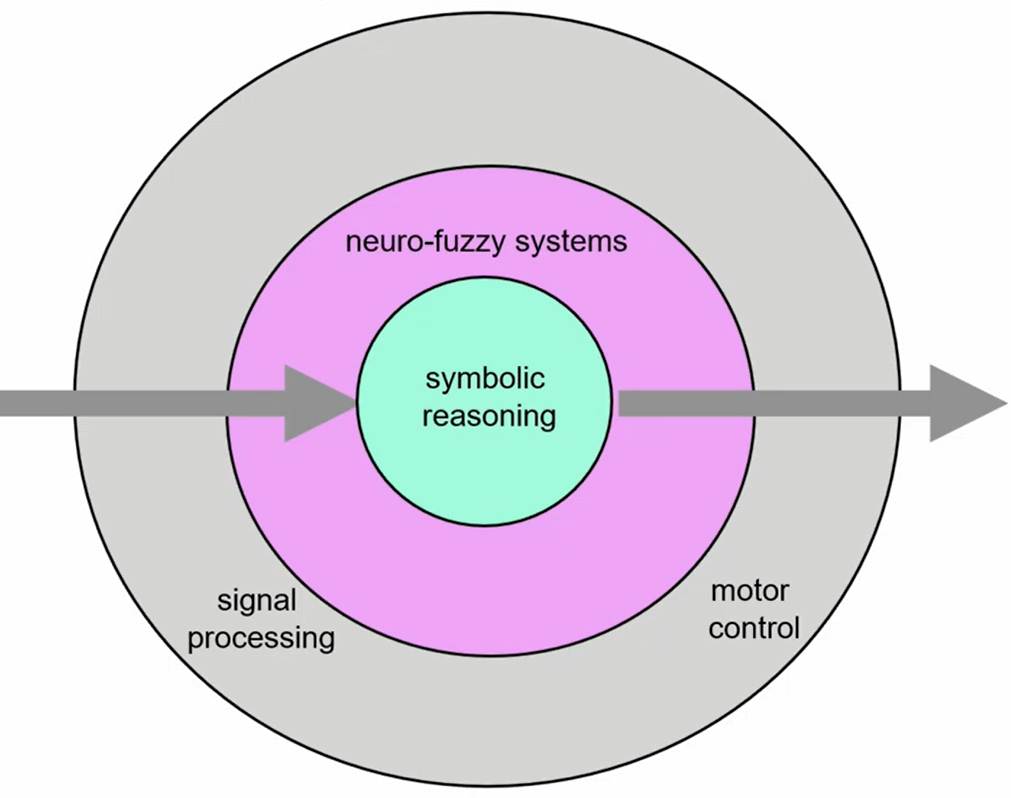
\includegraphics[width=0.5\linewidth]{Degree//static/AI_information_processing_view.png}
        \caption{Information Processing View of AI}
        \label{fig:AI-information-processing}
    \end{figure}
    \item \textbf{Intelligence}: \textbf{Remember the past and learn from it.} Memory and experience(case based reasoning), Learn a model(Machine learning), Recognize objects, faces, patterns(deep neural networks).\\
    \textbf{Understand the present. Be aware of the world around you.} Create a model of the world(knowledge representation), Make inferences from what you know(logic and reasoning).\\
    \textbf{Imagine the future. Work towards your goals.} Trial and error(heuristic search), Goals, plans, and actions(automated planning).
\end{itemize}

\subsection{Human Cognitive Architecture}
\begin{itemize}
    \item \textbf{Knowledge and Reasoning}: What does the agent know and what else does the agent know as a consequence of what it knows.
    \item \textbf{Semiotics}: A symbol is something that stands for something else. All languages, both spoken and written, are semiotic systems.
    \item \textbf{Biosemiotics}: How complex behaviour emerges when simple systems interact with each other through signs.
    \item \textbf{Reasoning}: The manipulation of symbols in a meaningful manner.
\end{itemize}

\subsection{Problem-Solving}
\begin{itemize}
    \item An autonomous agent in some world has a goal to achieve and a set of actions to choose from to strive for the goal.
    \item We deal with simple problems first, i.e., the world is static, the world is completely known, only one agent changes the world, action never fail, representation of the world is taken care of.
\end{itemize}

\section{Search Methods}

\subsection{State Space Search}
\begin{itemize}
    \item We start with the map coloring problem, where we want to color each region in the map with an allowed color such that no two adjacent regions have the same color.
    \begin{figure}[H]
        \centering
        \begin{subfigure}[b]{0.45\textwidth}
            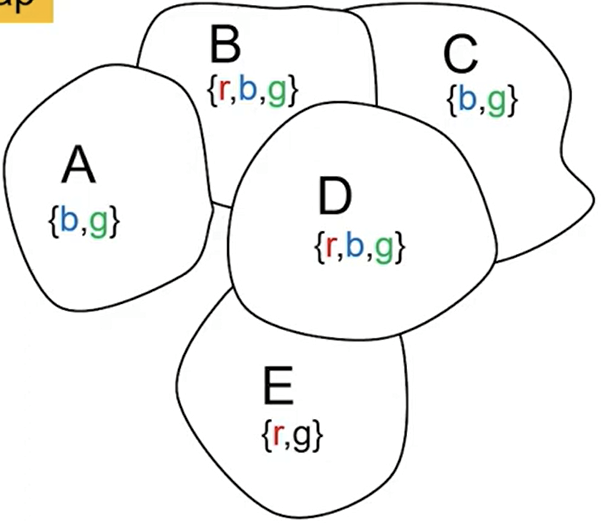
\includegraphics[width=1\textwidth]{Degree/static/AI_map_colors.png}
            \caption{Map with Constraints}
            \label{fig:AI-map-constraint}
        \end{subfigure}
        \hfill
        \begin{subfigure}[b]{0.45\textwidth}
            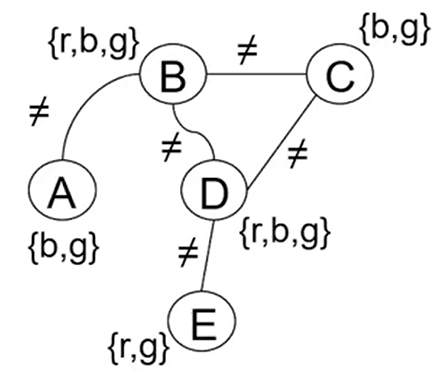
\includegraphics[width=1\textwidth]{Degree/static/AI_constraint_graph.png}
            \caption{Constraint Graph}
            \label{fig:AI-constraint-graph}
        \end{subfigure}
        \caption{Map Coloring Problem}
        \label{fig:AI-map-coloring-problem}
    \end{figure}
    \textbf{Brute Force}: Try all combinations of color for all regions.\\
    \textbf{Informed Search}: Choose a color that does not conflict with neighbors.\\
    \textbf{General Search}: Pose the problem to serve as an input to a general search algorithm.\\
    Map coloring can be posed as a constraint satisfaction problem or as a state space search, where the move is to assign a color to a region in a given partially colored state.
    \item \textbf{General Purpose methods}: Instead of writing a custom program for every problem to be solved, these aim to write search algorithms into which individual methods can be plugged in. One of them is State Space Search.
    \item \textbf{State or Solution Space Search}: Describe the given state, devise an operator to choose an action in each state, and then navigate the state space in search of the desired or goal state. Also known as Graph Search.\\
    A \textbf{state} is a representation of a situation.\\
    A \textit{MoveGen} function captures the moves that can be made in a given state.\\
    It returns a set of states - \textit{neighbors} - resulting from the moves.\\
    The state space is an implicit graph defined by the \textit{MoveGen} function.\\
    A \textit{GoalTest} function checks if the given state is a \textit{goal} state.\\
    A \textit{search algorithm} navigates the state space using these two functions.
    \item \textbf{The Water Jug Problem}: You have three jugs with capacity 8, 5 and 3 liters. Any state can be written as $[a,b,c]$, where $a,b,c$ are the amount of water present in each jug\\
    Start state: The 8-liter jug is filled with water, and the other two are empty, $[8,0,0]$. It can be seen that at any state the total amount of water remains the same.\\
    Goal: You are required to measure 4 liters of water. So, our goal state is $[4,x,y]$ or $[x,4,y]$ or $[x,y,4]$. A \textit{GoalTest} function can be written as
    \begin{algorithm}[H]
    \caption{GoalTest for the Water Jug Problem}\label{alg:AI-goal-test-water-jug}
        \begin{algorithmic}[1]
            \Require $[a,b,c]$, the state which needs to be checked
            \If{$a=4$ or $b=4$ or $c=4$}
                \State \Return True
            \EndIf
            \State \Return False
        \end{algorithmic}
    \end{algorithm}
    \item A few other examples are \textbf{The Eight Puzzle}, \textbf{The Man, Goat, Lion, Cabbage} and \textbf{The N-Queens Problem}.
\end{itemize}
Before studying different algorithms, we need to familiarize ourselves with some pseudocode syntax.

\subsection{General Search Algorithms}
\begin{itemize}
    \item Searching is like treasure hunting. Our approach would be to generate and test where we traverse the space by generating new nodes and test each node whether it is the goal or not.
    \item \textbf{Simple Search 1}: Simply pick a node N from OPEN and check if it is the goal.
    \begin{algorithm}[H]
        \caption{Simple Search 1}\label{alg:AI-simple-search-1}
        \begin{algorithmic}[1]
            \LComment{S is the initial state}
            \State OPEN $\gets \{S\}$
            \While{\textit{OPEN} is not empty}
                \State pick some node N from OPEN
                \State OPEN $\gets$ OPEN - $\{n\}$
                \If{\Call{GoalTest}{N} = True}
                    \State \Return N
                \Else
                    \State OPEN $\gets$ OPEN $\cup$ \Call{MoveGen}{N}
                \EndIf
            \EndWhile
            \State \Return FAILURE
        \end{algorithmic}
    \end{algorithm}
    This algorithm may run into an infinite loop, to address it we have \textbf{Simple Search 2}.
    \begin{algorithm}[H]
        \caption{Simple Search 2}\label{alg:AI-simple-search-2}
        \begin{algorithmic}[1]
            \LComment{S is the initial state}
            \State OPEN $\gets \{S\}$
            \State CLOSED $\gets \{\}$ 
            \While{\textit{OPEN} is not empty}
                \State pick some node N from OPEN
                \State OPEN $\gets$ OPEN - $\{n\}$
                \State CLOSED $\gets$ CLOSED $\cup$ $\{N\}$
                \If{\Call{GoalTest}{N} = True}
                    \State \Return N
                \Else
                    \State OPEN $\gets$ OPEN $\cup$ $\{$\Call{MoveGen}{N} - CLOSED$\}$
                \EndIf
            \EndWhile
            \State \Return FAILURE
        \end{algorithmic}
    \end{algorithm}
    We can modify this a bit further by doing, OPEN $\gets$ OPEN $\cup$ $\{$\textit{MoveGen(N)} - CLOSED - OPEN$\}$, this lowers the state space even more.
\end{itemize}

\subsection{Planning and Configuration Problems}
\begin{itemize}
    \item \textbf{Planning Problems}: Goal is known or describe, path is sought. Examples include River crossing problems, route finding etc.
    \item \textbf{Configuration Problems}: A state satisfying a description is sought. Examples include N-queens, crossword puzzle, Sudoku, etc.
    \item The simple search algorithms will work for configuration problems, but they won't return any path.
    \item \textbf{NodePairs}: Keep track of parent nodes. Each node is a pair $(currentNode,\text{ }parentNode)$.
    \item \textbf{Depth First Search}: OPEN is a stack data structure
    \begin{algorithm}[H]
        \caption{Depth First Search}\label{alg:AI-DFS}
        \begin{algorithmic}[1]
            \State OPEN $\gets$ (S, null) : [ ]
            \State CLOSED $\gets$ [ ]
            \While{OPEN is not empty}
                \State nodePair $\gets$ head OPEN
                \State (N, $\_$) $\gets$ nodePair
                \If{\Call{GoalTest}{N} = True}
                    \State \Return \Call{ReconstructPath}{nodePair, CLOSED}
                \EndIf
                \State CLOSED $\gets$ nodePair : CLOSED
                \State children $\gets$ \Call{MoveGen}{N}
                \State newNodes $\gets$ \Call{RemoveSeen}{children, OPEN, CLOSED}
                \State newPairs $\gets$ \Call{MakePairs}{newNodes, N}
                \State OPEN $\gets$ newPairs ++ tail OPEN
            \EndWhile
            \State \Return [ ]
            \Statex
            \Function{RemoveSeen}{nodeList, OPEN, CLOSED}
                \If{nodeList = [ ]}
                    \State \Return [ ]
                \EndIf
                \State node $\gets$ head nodeList
                \If{\Call{OccursIn}{node, OPEN} or \Call{OccursIn}{node, CLOSED}}
                    \State \Return \Call{RemoveSeen}{tail nodeList, OPEN, CLOSED}
                \EndIf
                \State \Return node : \Call{RemoveSeen}{tail nodeList, OPEN, CLOSED}
            \EndFunction
            \Statex
            \Function{OccursIn}{node, nodePairs}
                \If{nodePairs = [ ]}
                    \State \Return FALSE
                \ElsIf{node = first head nodePairs}
                    \State \Return TRUE
                \EndIf
                \State \Return \Call{OccursIn}{node, tail nodePairs}
            \EndFunction
            \Statex
            \Function{MakePairs}{nodeList, parent}
                \If{nodeList = [ ]}
                    \State \Return [ ]
                \EndIf
                \State \Return (head nodeList, parent) : \Call{MakePairs}{tail nodeList, parent}
            \EndFunction
            \Statex
            \Function{ReconstructPath}{nodePair, CLOSED}
                \State (node, parent) $\gets$ nodePair
                \State path $\gets$ node : [ ]
                \While{parent is not null}
                    \State path $\gets$ parent : path
                    \State CLOSED $\gets$ \Call{SkipTo}{parent, CLOSED}
                    \State($\_$, parent) $\gets$ head CLOSED
                \EndWhile
                \State \Return path
            \EndFunction
            \algstore{bkbreak}
        \end{algorithmic}
    \end{algorithm}
    \begin{algorithm}[H]
        \caption{Depth First Search continued}
        \begin{algorithmic}
            \algrestore{bkbreak}
            \Statex
            \Function{SkipTo}{parent, nodePairs}
                \If{parent = first head nodePairs}
                    \State \Return nodePairs
                \EndIf
                \State \Return \Call{SkipTo}{parent, tail nodePairs}
            \EndFunction
        \end{algorithmic}
    \end{algorithm}
    \item \textbf{Breadth First Search}: We use a queue for the OPEN set.
    \begin{algorithm}
        \caption{Breadth First Search}\label{alg:AI-BFS}
        \begin{algorithmic}
            \State OPEN $\gets$ (S, null) : [ ]
            \State CLOSED $\gets$ [ ]
            \While{OPEN is not empty}
                \State nodePair $\gets$ head OPEN
                \State (N, $\_$) $\gets$ nodePair
                \If{\Call{GoalTest}{N} = True}
                    \State \Return \Call{ReconstructPath}{nodePair, CLOSED}
                \EndIf
                \State CLOSED $\gets$ nodePair : CLOSED
                \State children $\gets$ \Call{MoveGen}{N}
                \State newNodes $\gets$ \Call{RemoveSeen}{children, OPEN, CLOSED}
                \State newPairs $\gets$ \Call{MakePairs}{newNodes, N}
                \LComment{This is the only line that is different, we now add newPairs at the end of the list}
                \State OPEN $\gets$ tail OPEN ++ newPairs 
            \EndWhile
            \State \Return [ ]
        \end{algorithmic}
    \end{algorithm}
    \item BFS always generates the shortest path, whereas DFS may not generate the shortest path.
    \item \textbf{Time Complexity}: Assume constant branching factor $b$ and assume the goal occurs somewhere at depth $d$. In the best case the goal would be the first node scanned at depth $d$ and in the worst case the goal would b3 the last node scanned.\\
    Best Case: $N_{DFS}=d+1$ and $N_{BFS}=\frac{b^{d}-1}{b-1}+1$\\
    Worst Case: $N_{DFS}=N_{BFS}=\frac{b^{d+1}-1}{b-1}$\\
    Average: $N_{DFS}\approx \frac{b^d}{2}$ and $N_{BFS}\approx \frac{b^d(b+1)}{2(b-1)}$, $N_{BFS}\approx N_{DFS}(\frac{b+1}{b-1})$
    \begin{table}[H]
        \centering
        \begin{tabular}{|c|c|c|}
            \hline
             & Depth First Search & Breadth First Search \\
             \hline
            Time & Exponential & Exponential\\
            \hline
            Space & Linear & Exponential\\
            \hline
            Quality of Solution & No guarantees & Shortest path\\
            \hline
            Completeness & Not for infinite search space & Guaranteed to terminate if solution path exists\\
            \hline
        \end{tabular}
        \caption{DFS vs BFS}
        \label{tab:AI-DFS-vs-BFS}
    \end{table}
    \item \textbf{Depth Bounded DFS}: Do DFS with a depth bound $d$. It is not complete and does not guarantee the shortest path. Given below is a modified version that returns the count of nodes visited, to get the original version just remove count.
    \begin{algorithm}[H]
        \caption{Depth Bounded DFS}\label{alg:AI-depth-DFS}
        \begin{algorithmic}[1]
            \State count $\gets$ 0
            \State OPEN $\gets$ (S, null, 0) : [ ]
            \State CLOSED $\gets$ [ ]
            \While{OPEN is not empty}
                \State nodePair $\gets$ head OPEN
                \State (N, $\_$, depth) $\gets$ nodePair
                \If{\Call{GoalTest}{N} = True}
                    \State \Return count, \Call{ReconstructPath}{nodePair, CLOSED}
                \EndIf
                \State CLOSED $\gets$ nodePair : CLOSED
                \If{depth $<$ depthBound}
                    \State children $\gets$ \Call{MoveGen}{N}
                    \State newNodes $\gets$ \Call{RemoveSeen}{children, OPEN, CLOSED}
                    \State newPairs $\gets$ \Call{MakePairs}{newNodes, N, depth + 1}
                    \State OPEN $\gets$ newPairs ++ tail OPEN
                    \State count $\gets$ count + length newPairs
                \Else
                    \State OPEN $\gets$ tail OPEN
                \EndIf
            \EndWhile
            \State \Return count, [ ]
        \end{algorithmic}
    \end{algorithm}
    \item \textbf{Depth First Iterative Deepening}: Iteratively increase depth bound. Combines best of BFS and DFS. This will give the shortest path, but we have to be careful that we take correct nodes from CLOSED. $N_{DFID}\approx N_{BFD}\frac{b}{b-1}$ for large $b$.
    \begin{algorithm}[H]
        \caption{Depth First Iterative Deepening}\label{alg:AI-depth-first-iterative}
        \begin{algorithmic}[1]
            \State count $\gets$ $-1$
            \State path $\gets$ [ ]
            \State depthBound $\gets$ $0$
            \Repeat
                \State previousCount $\gets$ count
                \State (count, path) $\gets$ \Call{DB-DFS}{$S,depthBound$}
                \State depthBound $\gets$ depthBound $+1$
            \Until{(path is not empty) or (previousCount $==$ count)}
            \State \Return path
        \end{algorithmic}
    \end{algorithm}
    \item DFID-C as compared to regular DFID-N adds new neighbors to OPEN list and also adds neighbors that are in CLOSED but not in OPEN list. This allows DFID-C to get the shortest path whereas DFID-N may not get the shortest path.
    \item The monster that AI fights is Combinatorial Explosion.
    \item All these algorithms we studied are blind algorithms or uniformed search, they don't know where the goal is.
\end{itemize}

\subsection{Heuristic Search}
\begin{itemize}
    \item Testing the neighborhood and following the steepest gradient identifies which neighbors are the lowest or closest to the bottom.
    \item The heuristic function $h(N)$ is typically a user defined function, $h(Goal)=0$.
    \item \textbf{Best First Search}: Instead of having a simple stack or queue we use a priority queue sorted based on heuristic function. Search frontier depends upon the heuristic function. If graph is finite then this is complete and quality of solution will head towards the goal but may not give the shortest path.
    \begin{algorithm}[H]
        \caption{Best First Search}\label{alg:AI-BestFS}
        \begin{algorithmic}[1]
            \State OPEN $\gets$ (S, null, h(S)) : [ ]
            \State CLOSED $\gets$ [ ]
            \While{OPEN is not empty}
                \State nodePair $\gets$ head OPEN
                \State (N, $\_$, $\_$) $\gets$ nodePair
                \If{\Call{GoalTest}{N} = True}
                    \State \Return \Call{ReconstructPath}{nodePair, CLOSED}
                \EndIf
                \State CLOSED $\gets$ nodePair : CLOSED
                \State children $\gets$ \Call{MoveGen}{N}
                \State newNodes $\gets$ \Call{RemoveSeen}{children, OPEN, CLOSED}
                \State newPairs $\gets$ \Call{MakePairs}{newNodes, N}
                \LComment{Again, this is pretty much the most important line}
                \State OPEN $\gets$ sort$_h$(newPairs ++ tail OPEN)
            \EndWhile
            \State \Return [ ]
        \end{algorithmic}
    \end{algorithm}
    \item For The eight puzzle we can define a few heuristic functions as follows:\\
    $h_1(n)=$ number of tiles out of place, Hamming distance.\\
    $h_2(n)=$ $\sum_{\text{for each tile}}$ Manhattan distance to its destination.
    \item \textbf{Hill Climbing}: A local search algorithm, i.e., move to the best neighbor if it is better, else terminate. In practice sorting is not needed, only the best node. This has burnt its bridges by not storing OPEN. We are interested in this because it is a constant space algorithm, which is a vast improvement on the exponential space for BFS and DFS. It's time complexity is linear. It treats the problem as an optimization problem.
    \begin{algorithm}[H]
        \caption{Hill Climbing}\label{alg:AI-hill-climbing}
        \begin{algorithmic}[1]
            \State node $\gets$ Start
            \State newNode $\gets$ head(sort$_h$(moveGen(node)))
            \While{ $h(newNode)<$ $h(node)$}
                \State node $\gets$ newNode
                \State newNode $\gets$ head(sort$_h$(moveGen(node)))
            \EndWhile
            \State \Return node
        \end{algorithmic}
    \end{algorithm}
\end{itemize}

\subsection{Escaping Local Optima}
\begin{itemize}
    \item \textbf{Solution Space Search}: Formulation of the search problem such that when we find the goal node we have the solution, and we are done.
    \item \textbf{Synthesis Methods}: Constructive methods. Starting with the initial state and build the solution state piece by piece.
    \item \textbf{Perturbation Methods}: Permutation of all possible candidate solutions.
    \item \textbf{SAT problem}: Given a boolean formula made up of a set of propositional variables $V=\{a,b,c,d,e,...\}$ each of which can be $true$ or $false$, or $1$ or $0$, to find an assignment of variables such that the given formula evaluates to $true$ or $1$.\\
    A SAT problem with $N$ variables has $2^N$ candidates.
    \item \textbf{Travelling Salesman Problem}: Given a set of cities and given a distance measure between every pair of cities, the task is to find a Hamiltonian cycle, visiting each city exactly once, having the least cost.
    \begin{enumerate}
        \item \textbf{Nearest Neighbor Heuristic}: Start at some city, move to nearest neighbor as long as it does not close the loop prematurely.
        \item \textbf{Greedy Heuristic}: Sort the edges, then add the shortest available edge to the tour as long as it does not close the loop prematurely.
        \item \textbf{Savings Heuristic}: Start with $n-1$ tours of length $2$ anchored on a base vertex and performs $n-2$ merge operations to construct the tour.
        \item \textbf{Perturbation operators}: Start with some tour, then choose two cities and interchange, this gives the solution space. Heuristic function is $saving$ = $cost(base,a)$ + $cost(base,b)$ - $cost(a,b)$
        \item \textbf{Edge Exchange}: Similar to above but now instead of choosing cities we are choosing edges. Can be $2$-edge exchange, $3$-edge, $4$-edge, etc. City exchange is a special case of $4$-edge exchange.
    \end{enumerate}
    \item Solution space of TSP grows in order factorial, much faster than SAT problem.
    \item A collection of problems with some solutions is available \href{http://comopt.ifi.uni-heidelberg.de/software/TSPLIB95/}{here}.
    \item To escape local minima we need something called \textbf{exploration}.
    \item \textbf{Beam Search}: Look at more than one option at each level. For a beam width $b$, look at best $b$ options. Heavily memory dependent.
    \begin{algorithm}
        \caption{Beam Search}\label{alg:Beam-Search}
        \begin{algorithmic}
            \Statex \Call{BeamSearch}{$S,w$}
            \State OPEN $\gets$ $[S]$
            \State $N$ $\gets$ $S$
            \Do
                \State $bestEver$ $\gets$ $N$
                \If{\Call{Goal-Test}{OPEN} = True}
                    \State \Return goal from OPEN
                \EndIf
                \State $neighbors$ $\gets$ \Call{MoveGen}{OPEN}
                \State OPEN $\gets$ take w $sort_h(neighbors)$
                \State $N$ $\gets$ head(OPEN)
            \doWhile{$h(N)$ is better than $h(bestEver)$}
            \State \Return $bestEver$
        \end{algorithmic}
    \end{algorithm}
    \item \textbf{Variable Neighborhood Descent}: Essentially we are doing hill climbing with different neighborhood functions. The idea is to use sparse functions before using denser functions, so the storage is not high. The algorithm assumes that there are $N$ $moveGen$ functions sorted according to the density of the neighborhoods produced.
    \begin{algorithm}[H]
        \caption{Variable Neighborhood Descent}\label{alg:Variable-Neighborhood-Descent}
        \begin{algorithmic}[1]
            \Statex \Call{VariableNeighbourhoodDescent}{ }
            \State $node\gets$ $start$
            \For{$i\gets$ $1$ to $n$}
                \State $moveGen\gets$ \Call{MoveGen}{$i$}
                \State $node\gets$ \Call{HillClimbing}{$node,moveGen$}
            \EndFor
            \State \Return $node$
        \end{algorithmic}
    \end{algorithm}
    \item \textbf{Best Neighbor}: Another variation of Hill Climbing, simply move to the best neighbor regardless of whether it is better than current node or not. This will require an external criterion to terminate. It will not escape local maxima, as once it escapes it will go right back to it in the next iteration.
    \begin{algorithm}[H]
        \caption{Best Neighbor}\label{alg:best-neighbor}
        \begin{algorithmic}[1]
            \Statex \Call{BestNeighbor}{ }
            \State $N\gets$ $start$
            \State $bestSeen\gets$ $N$
            \While{some termination criterion}
                \State $N\gets$ \Call{best}{$moveGen(N)$}
                \If{$N$ better than $bestSeen$}
                    \State $bestSeen\gets$ $N$
                \EndIf
            \EndWhile
            \State \Return $bestSeen$
        \end{algorithmic}
    \end{algorithm}
    \item \textbf{Tabu Search}: Similar to Best Neighbor but not allowed back immediately. An aspiration criterion can be added that says that if a tabu move result in a node that is better than bestSeen then it is allowed. To drive this search into newer areas, keep a frequency array and give preference to lower frequency bits or bits that have been changed less.
    \begin{algorithm}[H]
        \caption{Tabu Search}\label{alg:tabu-search}
        \begin{algorithmic}[1]
            \Statex \Call{TabuSearch}{ }
            \State $N\gets$ $start$
            \State $bestSeen\gets$ $N$
            \While{some termination criterion}
                \State $N\gets$ \Call{best}{\Call{allowed}{$moveGen(N)$}}
                \If{$N$ better than $bestSeen$}
                    \State $bestSeen\gets$ $N$
                \EndIf
            \EndWhile
            \State \Return $bestSeen$
        \end{algorithmic}
    \end{algorithm}
\end{itemize}

\section{Stochastic Search}
Very often to escape local minima we use Stochastic/Randomized methods instead of Deterministic methods.
\subsection{Iterated Hill Climbing}
\begin{itemize}
    \item \textbf{2SAT}: Problems where each clause has at most two literals, known to be solved in polynomial time. However, if we add even 1 more literal it would become NP-complete or exponential.
    \item Iterated hill climbing says that we should perform hill climbing with multiple different starting nodes chosen randomly to have a higher probability of finding the goal node.
    \begin{algorithm}[H]
        \caption{Iterated Hill Climbing}\label{alg:AI-iterated-hill-climbing}
        \begin{algorithmic}[1]
            \Statex \Call{Iterated-Hill-Climbing}{$N$}
            \State $bestNode$ $\gets$ \textbf{random candidate solution}
            \For{$i\gets$ $1$ to $N$}
                \State $currentBest$ $\gets$ \Call{Hill-Climbing}{\textbf{new random candidate solution}}
                \If{$h(currentBest)$ is better than $h(bestNode)$}
                    \State $bestNode$ $\gets$ $currentBest$
                \EndIf
            \EndFor
            \State \Return $bestNode$
        \end{algorithmic}
    \end{algorithm}
\end{itemize}

\subsection{Stochastic Actions}
\begin{itemize}
    \item To move or not to move is the question.
    \item Idea is we would like to consider actions that are good in terms of heuristic functions, but sometimes we even want to move when heuristic function is not necessarily good.
    \item \textbf{Random Walk}: Choose a random node and move there, hill climbing of stochastic search.
    \begin{algorithm}[H]
        \caption{Random Walk}\label{alg:AI-random-walk}
        \begin{algorithmic}[1]
            \Statex \Call{RandomWalk}{ }
            \State $node$ $\gets$ random candidate solution or start
            \State $bestNode$ $\gets$ $node$
            \For{$i\gets$ $1$ to $n$}
                \State $node$ $\gets$ \Call{RandomChoose}{\Call{MoveGen}{$node$}}
                \If{$node$ is better than $bestNode$}
                    \State $bestNode$ = $node$
                \EndIf
            \EndFor
        \end{algorithmic}
    \end{algorithm}
    \item \textbf{Stochastic Hill Climbing}: Let the algorithm be at the current bode $v_c$, then we select a random neighbor $v_N$ and calculate $\Delta E=(eval(v_N)-eval(v_c))$.\\
    If $\Delta E$ is positive, it means that $v_N$ is better than $v_c$, then the algorithm should move to it with a higher probability.\\
    If $\Delta E$ is negative, it means that $v_N$ is better than $v_c$, then the algorithm should move to it with a lower probability.\\
    The probability is computed using the sigmoid function, which is given as
    \begin{equation*}
        \text{Probability }P=\frac{1}{1+e^{-\frac{\Delta E}{T}}}
    \end{equation*}
    where $T$ is a parameter. The algorithm essentially combines exploration with exploitation.
    \item \textbf{Annealing}: In metallurgy and materials science, \textbf{annealing} is a heat treatment that alters the physical and sometimes chemical properties of a material to increase its ductility and reduce its hardness, making it more workable. It involves heating a material above its recrystallization temperature, maintaining a suitable temperature for an appropriate amount of time and then cooling.\\
    In annealing, atoms migrate in the crystal lattice and the number of dislocations decreases, leading to a change in ductility and hardness. As the material cools it recrystallizes.
    \item \textbf{Simulated Annealing}: Essentially tries to mimic the annealing process, begins with exploration and ends with exploitation. Annealing is also where $\Delta E$ and $T$ come from, essentially meaning Energy and Temperature.
    \begin{algorithm}[H]
        \caption{Simulated Annealing}\label{alg:simulated-annealing}
        \begin{algorithmic}[1]
            \Statex \Call{SimulatedAnnealing}{ }
            \State $node\gets$ random candidate solution or start
            \State $bestNode\gets$ $node$
            \State $T\gets$ some large value
            \For{$time\gets$ $1$ to $numberOfEpochs$}
                \While{some termination criteria} \Comment{$M$ cycles in a sample case}
                    \State $neighbor\gets$ \Call{RandomNeighbor}{$node$}
                    \State $\Delta E\gets$ $Eval(neighbor)-Eval(node)$
                    \If{$Random(0,1)<$ \Call{Sigmoid}{$\Delta E, T$}}
                        \State $node\gets$ $neighbor$
                        \If{$Eval(node)>Eval(bestNode)$}
                            \State $bestNode\gets$ $node$
                        \EndIf
                    \EndIf
                \EndWhile
                \State $T\gets$ \Call{CoolingFunction}{$T,times$}
            \EndFor
            \State \Return $bestNode$
        \end{algorithmic}
    \end{algorithm}
\end{itemize}

\subsection{Genetic Algorithms}
\begin{itemize}
    \item Survival of the fittest. Inspired by the process of natural selection.
    \item A class of methods for optimization problems, more generally known as Evolutionary Algorithms.
    \item Implemented on a population of candidates in the solution space. A fitness function evaluates each candidate. The fittest candidates get to mate and reproduce.
    \item \textbf{Artificial Selection}: Given a population of candidate solutions we do a three step iterative process
    \begin{enumerate}
        \item \textbf{Reproduction}: Clone each candidate in proportion to its fitness. Some may get more than one copy, some none.
        \item \textbf{Crossover}: Randomly mate the resulting population and mix up the genes.
        \item \textbf{Mutation}: Once in a while, in search of a missing gene.
    \end{enumerate}
    \item \textbf{Selection}: Imagine a roulette wheel on which each candidate in the parent population $\{P_1,P_2,...,P_N\}$ is represented as a sector. The angle subtended by each candidate is proportional to its fitness. The roulette wheel is spun $N$ times. Then the selected parents are added one by one to create a new population.
    \item \textbf{Crossover Operators}: A \textit{single point crossover} simply cuts the two parents at a randomly chosen point and recombines them to form two new solution strings. It can be at multiple points as well, idea is to mix up the genes.
    \begin{algorithm}[H]
        \caption{Genetic Algorithm}\label{alg:genetic-algorithm}
        \begin{algorithmic}[1]
            \Statex \Call{Genetic-Algorithm}{ }
            \State $P\gets$ create $N$ candidate solutions \Comment{initial population}
            \Repeat
                \State compute fitness value for each member of $P$
                \State $S\gets$ with probability proportional to fitness value, randomly select $N$ member from $P$.
                \State $offspring\gets$ partition $S$ into two halves, and randomly mate and crossover members to generate $N$ offsprings.
                \State With a low probability mutate some offsprings
                \State Replace $k$ the weakest members of $P$ with $k$ strongest offsprings
            \Until{some termination criteria}
            \State \Return the best member of $P$
        \end{algorithmic}
    \end{algorithm}
    \item A large diverse population size is necessary for the performance of genetic algorithm to work.
    \item One issue is how to represent candidate solutions?, as they can be of any type. One simple solution is to convert the solution into a string this will require an additional function.
    \item In TSP, one problem is also that during crossover some cities can get repeated.
    \item \textbf{Cycle Crossover}: Identify cycles, look at below image, easier to understand.
    \begin{figure}[H]
        \centering
        \begin{subfigure}[b]{0.45\textwidth}
            \centering
            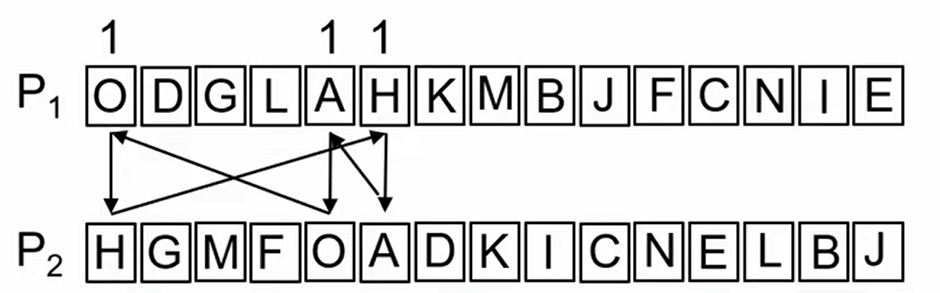
\includegraphics[width=\textwidth]{Degree//static/AI_TSP_ga_cycle1.png}
            \caption{TSP cycle 1}
        \end{subfigure}
        \hfill
        \begin{subfigure}[b]{0.45\textwidth}
            \centering
            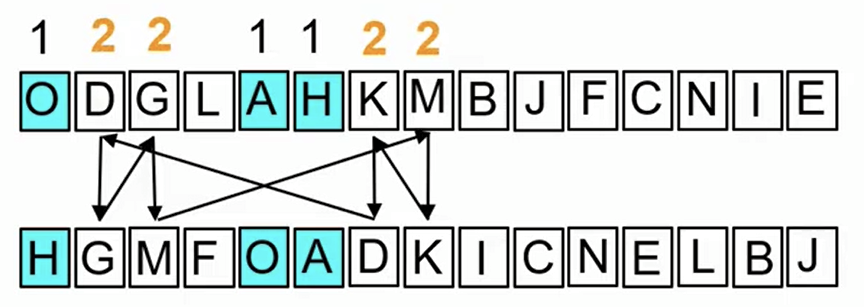
\includegraphics[width=\textwidth]{Degree//static/AI_TSP_ga_cycle2.png}
            \caption{TSP cycle 2}
        \end{subfigure}
        \caption{TSP Identifying cycles}
    \end{figure}
    Once cycles are identified, then $C_1$ gets odd numbered cycles from $P_1$ and even numbered cycles from $P_2$ the other go to $C_2$.
    \item \textbf{Partially Mapped Crossover(PMX)}: Identify some cities that form a subtour and establish a mapping.
    \begin{figure}[H]
        \centering
        \begin{subfigure}[b]{0.45\textwidth}
            \centering
            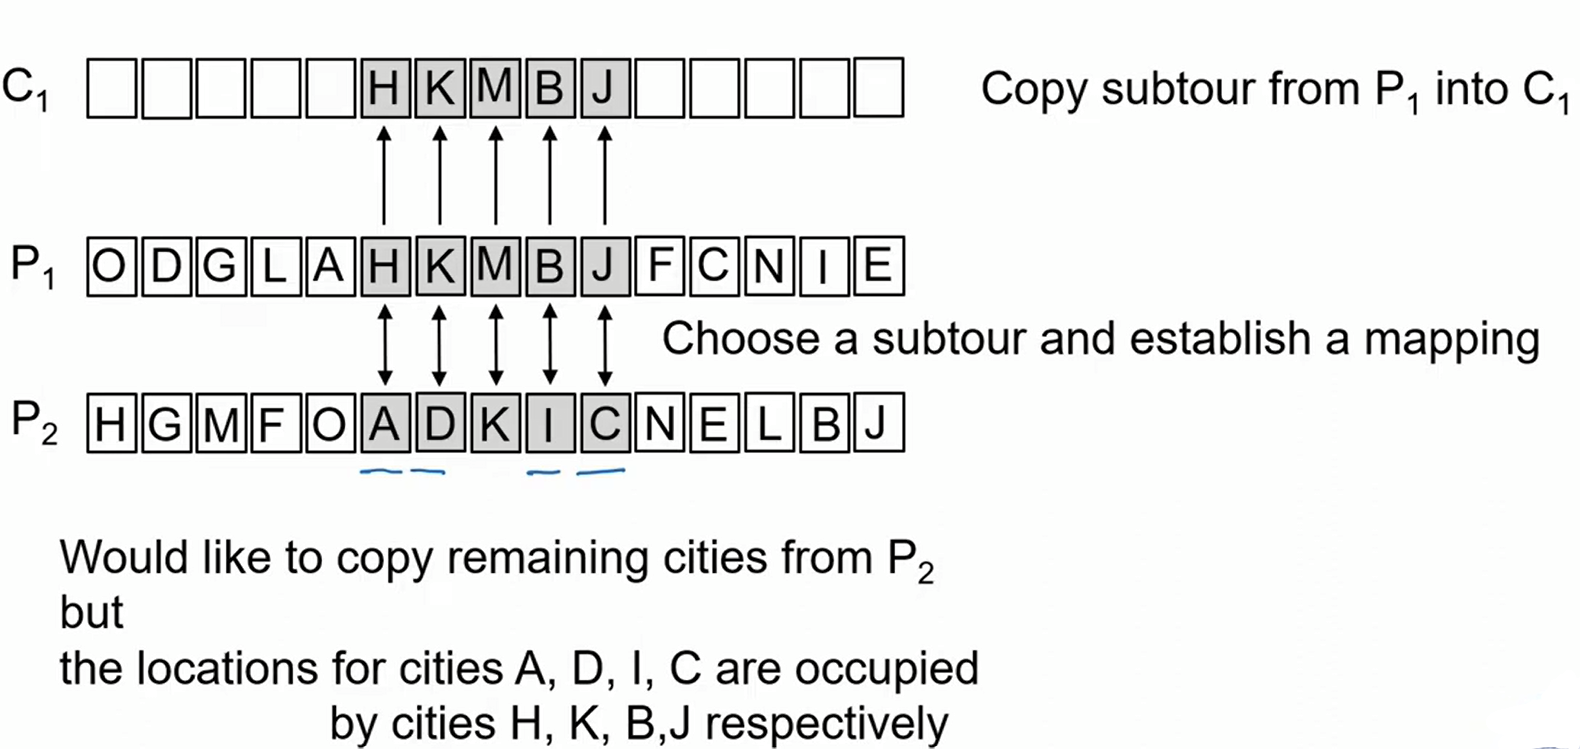
\includegraphics[width=\textwidth]{Degree/static/AI_TSP_partialcrossover_subtour.png}
            \caption{Choose Subtour}
        \end{subfigure}
        \hfill
        \begin{subfigure}[b]{0.45\textwidth}
            \centering
            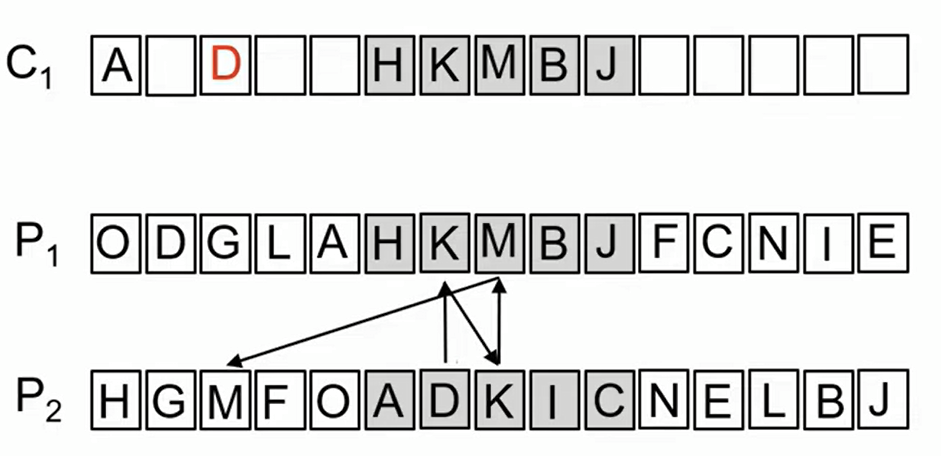
\includegraphics[width=\textwidth]{Degree/static/AI_TSP_partialcrossover_rest.png}
            \caption{Copy occupied spaces}
        \end{subfigure}
        \caption{Partially Mapped Crossover}
    \end{figure}
    \item \textbf{Order Crossover}: Copy a subtour from $P_1$ into $C_1$ and the remaining from $P_2$ in the order they occur in $P_2$.
    \item For all the above we were using path representation of TSP, there is another representation of TSP.
    \item \textbf{Adjacency Representation}: The cities are arranged based on where they come from in the tour with respect to the index. For example if $A\rightarrow H$, then at index 0 we would have $H$.
    \item \textbf{Alternating Edges Crossover}: From a given city $X$ choose the next city $Y$ from $P_1$ and from the city $Y$ choose the next city from $P_2$ and so on. It is possible to run into cycles, need to be careful.
    \item \textbf{Heuristic Crossover}: For each city choose the next from that parent $P_1$ or $P_2$ whichever is closer.
    \item \textbf{Ordinal Representation}: Replace the name of the city is Path Representation one by one to its current numeric index. At the start all cities $A,B,C,D,E$ will have numeric index $1,2,3,4,5$, now consider if we add $C$ to the representation the new indexing would be for cities $A,B,D,E$, we have $1,2,3,4$. The \textbf{advantage} is that single point crossover produces valid offspring.
\end{itemize}

\subsection{Ant Colony Optimization}
\begin{itemize}
    \item \textbf{Emergent Systems}: Collections of simple entities organize themselves and a larger more sophisticated entity emerges. The behavior of this complex system is a property that emerges from interactions amongst its components.
    \item \textbf{Conway's Game of Life}: A cellular automaton in which cells are alive or dead. Each cell obeys the following rules to decide its fate in the next time step.
    \begin{table}[H]
        \centering
        \begin{tabular}{|c|c|c|}
            \hline
            Cell state & Number of alive neighbors & New cell state \\
            \hline
            alive & $<2$ & dead \\
            \hline
            alive & 2 or 3 & alive \\
            \hline
            alive & $>3$ & dead \\
            \hline
            dead & 3 & alive \\
            \hline
        \end{tabular}
        \caption{Rules for Game of Life}
        \label{tab:AI-rules-game-life}
    \end{table}
    \item Illusion of movement can be seen in an example called \textbf{Gosper's Glider Gun}.
    \item \textbf{Chaos and Fractals}: A fractal is a never-ending pattern. Fractals are infinitely complex patterns that are self-similar across different scales. They are created by repeating a simple process over and over in an ongoing feedback loop. Drive by recursion, fractals are images of dynamic systems, the pictures of chaos.
    \item Let 5 ants $A,B,C,D,$ and $E$ go out in search for food. Each ant lays a trail of pheromone where it goes. Each ant lays a trail of pheromone where it goes. More ants that emerge will tend to follow some pheromone trail.
    \item Let's say $A$ finds some food, then it will follow its pheromone trail back and the other ants will continue their search.
    \item Eventually, as more ants travel on the trail they deposit more pheromone and the trail gets stronger and stronger, eventually becoming the caravan we might have seen raiding our food. 
    \item They tend to find the shortest path.
    \item \textbf{Ant Colony Optimization}: We try to capitalize on this method. Each ant constructs a solution using a stochastic greedy method using a combination of a heuristic function and pheromone trail following.
    \item This is related to the class of algorithms known as \textit{Swarm Optimization}.
    \begin{algorithm}[H]
        \caption{Ant Colony Optimization for TSP}\label{alg:AI-ant-colony-tsp}
        \begin{algorithmic}[1]
            \Statex \Call{TSP-ACO}{ }
            \State $bestTour\gets$ NIL
            \Repeat
                \State randomly place $M$ ants on $N$ cities
                \For{each ant $a$}
                    \For{$n\gets$ $1$ to $N$}
                        \State ant $a$ selects an edge from the distribution $P_n^a$
                    \EndFor
                \EndFor
                \State update $bestTour$
                \For{each ant $a$}
                    \For{each edge $(u,v)$ in the ant's tour}
                        \State deposit pheromone $\propto$ 1/tour-length on edge $(u,v)$
                    \EndFor
                \EndFor
            \Until{some termination criteria}
            \State \Return $bestTour$
        \end{algorithmic}
    \end{algorithm}
    \item From a city $i$ the $k^{th}$ ant moves to city $j$ with a probability given by
    \begin{equation*}
        P^k_{ij}(t)=\begin{cases}
            \frac{[\tau_{ij}(t)]^\alpha \times [\eta_{ij}]^\beta}{\sum_{h\in allowed_k(t)}([\tau_{ih}(t)]^\alpha [\eta_{ih}(t)]^\beta)},\text{ if }j\in allowed_k(t)\text{ the cities ant }k\text{ is allowed to move to}\\
            0,\text{ otherwise}
        \end{cases}
    \end{equation*}
    where $\tau_{ij}(t)$ is pheromone on edge$_{ij}$ and $\eta_{ij}$ is called visibility which is inversely proportional to the distance between cities $i$ and $j$.
    \item After constructing a tour in $n$ time steps, each ant $k$ deposits an amount of pheromone $\frac{Q}{L_k}$ on the edges it has traversed, which is inversely proportional to the cost of the tour $L_k$ it found.
    \item Total pheromone deposited on edge$_{ij}$ is $\Delta \tau_{ij}(t,t+n)$
    \item The total pheromone on edge$_{ij}$ is updated as
    \begin{equation*}
        \tau_{ij}(t+n)=(1-\rho)\times \tau_{ij}(t)+\Delta \tau_{ij}(t,t+n)
    \end{equation*}
    where $\rho$ is the rate of evaporation of pheromone.
\end{itemize}

\section{Finding Optimal TSP Tours}
\subsection{Finding Optimal Paths}
\begin{itemize}
    \item Breadth First Search finds a solution with the smallest \textit{number} of moves. But if \textit{cost} of all moves is no the same then an \textbf{optimal} solution may not be the one with the smallest number of moves.
    \item \textbf{Brute Force}: Simply search the entire search tree, computationally it is mindlessly expensive.
    \item \textbf{Goal}: Search as little of the space as possible while guaranteeing the optimal solution.
    \item A \textit{Best First} approach to solving problems. Given a set of candidates a search algorithm has to choose from. Each candidate is tagged with an estimated cost of the complete solution.
    \item Branch and Bound in a refinement space
    \begin{enumerate}
        \item Initial solution set contains all solutions.
        \item In each step we partition a set into two smaller sets.
        \item Until we can pick a solution that is fully specified.
        \item Each solution set needs to have an estimated cost.
        \item B\&B will refine the solution that has the least estimated cost.
    \end{enumerate}
    \item An optimal solution can be guaranteed by ensuring that the estimated cost is a lower bound on actual cost.
    \item \textbf{Lower bound}: A solution will never be cheaper than it is estimated to be.
    \item Thus if a fully refined solution is cheaper than a partially refined one, the latter need not be explored - \textbf{PRUNING}. The higher the estimate, the better the pruning.
    \item Branch and Bound for TSP
    \begin{enumerate}
        \item Let the candidate solutions be permutations of the list of city names.
        \item The initial set of candidates includes all permutations.
        \item Refine the cheapest set by specifying a specific segment.
        \item Heuristic: Choose the segment with minimum cost.
        \item For tighter estimates, edges that cause three or more segment cycles are avoided.
        \item We, can also exclude an edge that is a third edge for a node, because a city has only two neighbors in a tour.
        \item Higher estimates require more work.
    \end{enumerate}
    \item A lower bound estimate could be for each row add up the smallest two positive entries and divide by two. This may not feasible.
    \item The basic idea behind B\&B is to prune those parts of a search space which cannot contain a better solution.
    \item Each candidate is tagged with an estimated cost of the complete solution.
    \item \textbf{Dijkstra's Algorithm}
    \begin{enumerate}
        \item Begins by assigning infinite cost estimates to all nodes except the start node.
        \item It assigns color white to all the nodes initially.
        \item It picks the cheapest white node and colors it black.
        \item \textbf{Relaxation}: Inspect all neighbors of the new black node and check if a cheaper path has been found to them.
        \item If yes, then update cost of that node, and mark the  parent node.
    \end{enumerate}
\end{itemize}

\subsection{Algorithm A*}
\begin{itemize}
    \item A* achieves better performance by using heuristics to guide its search.
    \item For all nodes we will compute $f(n)$ which is made up of two components $g(n)$ and $h(n)$.
    \item $g(n)$ = actual cost of solution found from the start node to node $n$.
    \item $h(n)$ = estimated cost of the path from node $n$ to goal node.
    \item Maintain a priority queue of nodes sorted on the $f$ values
    \item Pick the lowest $f$ value node, and check whether it is the goal node.
    \item Else generate its neighbors, and compute their $f$ values
    \item Insert new nodes into the priority queue
    \item For existing nodes check for better path(like Dijkstra's algorithm)
    \begin{algorithm}[H]
        \caption{A* Algorithm}\label{alg:AI-A*}
        \begin{algorithmic}[1]
            \Statex \Call{A*}{S}
            \State default value of $g$ for every node is $+\infty$
            \State $parent(S)\gets null$
            \State $g(S)\gets 0$
            \State $f(S)\gets g(S)+h(S)$
            \State $OPEN\gets$ $S:$[ ]
            \State $CLOSED\gets$ empty list
            \While{$OPEN$ is not empty}
                \State $N\gets$ remove node with the lowest $f$ value from $OPEN$
                \State add $N$ to CLOSED
                \If{\Call{GoalTest}{$N$}}
                    \State \Return \Call{ReconstructPath}{$N$}
                \EndIf
                \For{each neighbor $M\in $ \Call{MoveGen}{$N$}}
                    \If{$g(N)+k(N,M)<g(M)$}
                        \State $parent(M)\gets N$
                        \State $g(M)\gets g(N)+k(N,M)$
                        \State $f(M)\gets g(M)+h(M)$
                        \If{$M\in OPEN$} 
                            \State continue 
                        \EndIf
                        \If{$M\in CLOSED$} 
                            \State \Call{Propagate-Improvement}{$M$}
                        \Else 
                            \State add $M$ to $OPEN$ 
                        \EndIf
                    \EndIf
                \EndFor
            \EndWhile
            \Return empty list
        \end{algorithmic}
    \end{algorithm}
    \item Propagate improvement simply does line 13 to 17 recursively.
    \item A* is admissible if
    \begin{enumerate}
        \item The branching factor is finite, otherwise you cannot even generate the neighbors.
        \item Every edge has a cost greater than a small constant $\epsilon$, however it is possible to get stuck in an infinite path with a finite cost.
        \item For all nodes $h(n)\leq h^*(n)$
    \end{enumerate}
    \item If a path exists to the goal node, then the OPEN list always contains a node $n'$ from an optimal path. Moreover, the $f$ value of that node is not greater than the optimal value.
\end{itemize}

\subsection{Weighted A*}
\begin{itemize}
    \item $f(n)=g(n)+wh(n)$, where $w$ determines how much weight we give to the heuristic function.
    \item $w=0$, with the \textbf{pull} of the source being the dominating factor and only shortest path in mind.
    \item $w\to \infty$, with the \textbf{push} towards the goal being the dominating factor and only speed termination in mind.
    \item Best First Search and Weighted $A^*$ head off towards the goal directly.
    \item Branch and Bound and $A^*$ keep checking if a cheaper path is available.
    \item $w=0$ is essentially branch and bound, and $w\to \infty$ is essentially the best first search.
\end{itemize}

\subsection{A* Space Saving Versions}
\begin{itemize}
    \item \textbf{Iterative Deepening $A^*$}: Similar to DFID, but instead of having a depth parameter, we set the depth as $f$-values, initially set the bound as $f(S)$ which is equal to $h(S)$. In subsequent cycles it extends the bound to the next unexplored $f$-value.
    \begin{algorithm}[H]
        \caption{Iterative Deepening $A^*$}
        \begin{algorithmic}[1]
            \Statex \Call{IterativeDeepeningA*}{$start$}
            \State $depthBound\gets f(S)$
            \While{$TRUE$}
                \State \Call{DepthBoundedDFS}{$start,depthBound$}
                \State $depthBound\gets f(N)$ of cheapest unexpanded node on $OPEN$
            \EndWhile
        \end{algorithmic}
    \end{algorithm}
    \item Even when the state space grows quadratically the number of paths to each node grows exponentially.
    \item The DFS algorithm can spend a lot of time exploring these different paths if a CLOSED list is not maintained. The other problem is that in each cycle it extends the bound only to the next $f$-value.
    \item IDA* has linear space requirements however has no sense of direction.
    \item \textbf{Recursive best first search} is a linear space best-first search algorithm, will expand fewer nodes than iterative deepening with a non-decreasing cost function. This is like Hill Climbing with backtracking.
    \item Backtrack if \textit{no child} is the best node on OPEN, except RBFS \textit{rolls} back search to a node it has marked as second best. While rolling back it backs up the lowest value for each node on from its children to update the value of the parent.
    \item \textbf{The Monotone Condition}: Says that for a node $n$ that is a successor to a node $m$ on a path to the goal being constructed by the algorithm $A^*$ using the heuristic function $h(x)$,
    \begin{equation*}
        h(m)-h(n)\leq k(m,n)
    \end{equation*}
    The heuristic function underestimates the cost of each edge.
    \begin{equation*}
        h(m)+g(m)\leq k(m,n)+h(n)+g(m) = h(n)+g(n)
    \end{equation*}
    For $A^*$ the interesting consequence of searching with a heuristic function satisfying the monotone property is that every time it picks a node for expansion, it has found an optimal path to that node.\\
    As a result, there is no necessity of improved cost propagation through nodes in CLOSED.
\end{itemize}

\subsection{Pruning in A*}
\begin{itemize}
    \item \textbf{Sequence Alignment Problem}: Finding the similarity of two amino acid sequences.
    \item Given two sequences compose of the characters $C,A,G$ and $T$ the task of sequence alignment is to list the two alongside with the option of inserting a gap in either sequence. The objective is to maximize the similarity between the resulting two sequences with gaps possibility inserted.
    \item The similarity can be quantified by associating a cost with misalignment. Typically, two kinds of penalties are involved\\
    \textbf{Mismatch}: If character $X$ is aligned to a different character $Y$.\\
    \textbf{Indel}: associated with inserting a gap.
    \item \textbf{Similarity function}: A similarity function is a kind of \textit{inverse} of the distance function. Using a similarity function transforms the sequence alignment into a \textit{maximization} problem.
    \item Let $X$ and $Y$ be the first characters of the two strings. There are three possibilities
    \begin{enumerate}
        \item Align $X$ with $Y$
        \item Insert blank before $X$
        \item Insert blank before $Y$
    \end{enumerate}
    \begin{figure}[H]
        \centering
        \begin{subfigure}[b]{0.45\linewidth}
            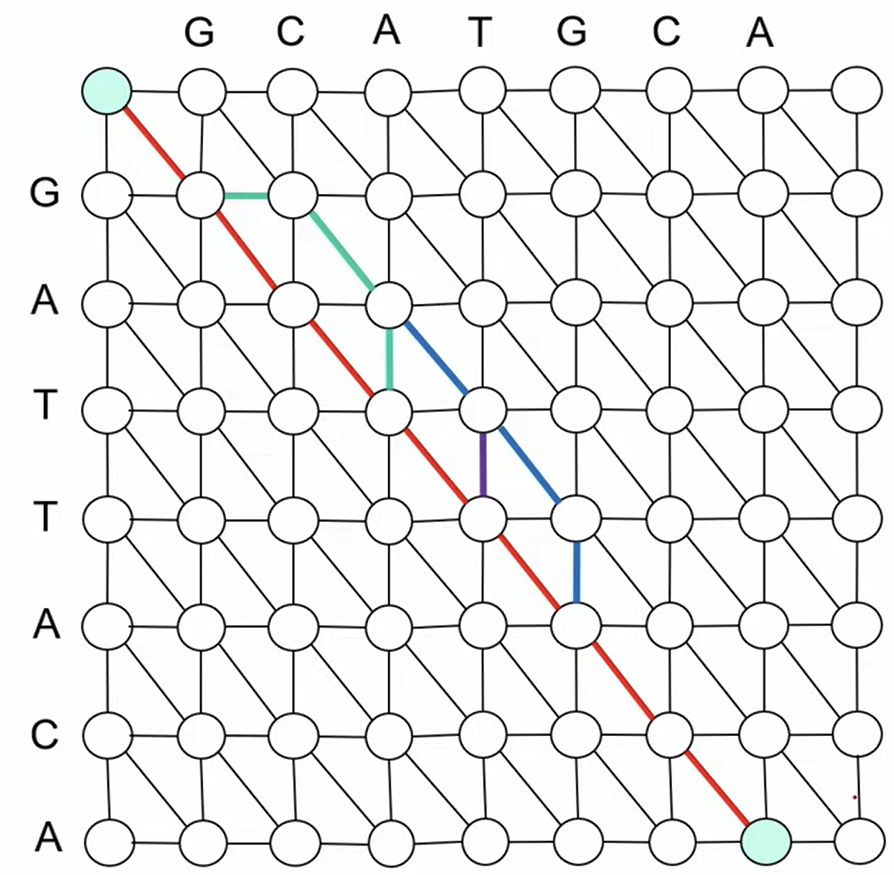
\includegraphics[width=\textwidth]{Degree//static/AI_sequence_alignment.png}
        \end{subfigure}
        \hfill
        \begin{subfigure}[b]{0.45\linewidth}
            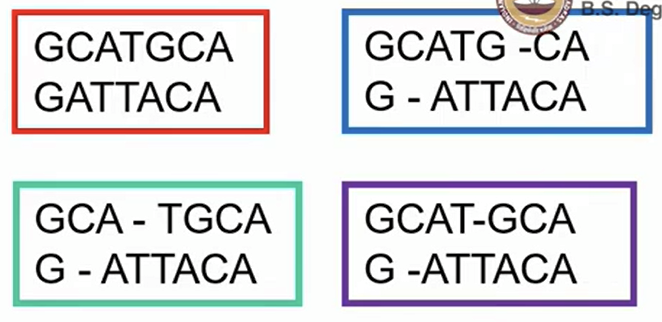
\includegraphics[width=\textwidth]{Degree//static/AI_sequence_path.png}
        \end{subfigure}
        \caption{Sequence Alignment Graph}
        \label{fig:AI-sequence-alignment}
    \end{figure}
    \item OPEN grows linearly, whereas CLOSED grows quadratically.
    \item \textbf{Frontier Search}: Only maintain OPEN and throw away CLOSED, nodes in OPEN will be \textbf{barred} from generating nodes that would have been in CLOSED. Search only moves forward, without "leaking back".It has no means of reconstructing the optimal path it has found.
    \item \textbf{Relay nodes}: at roughly the halfway mark. When a node on OPEN has $g(n)\approx h(n)$ mark it as relay and keep pointers from its descendants on OPEN.
    \item Now solve two recursive problems, from start to relay and from relay to goal.
    \item This is known as \textbf{Divide and Conquer Frontier Search}(DCFS).
    \item \textbf{Smart Memory Graph Search (SMGS)}: Given that memory is getting cheaper and abundant, one \textit{need not} make recursive calls when $A^*$(without pruning) could have solved the problem. Keep track of available memory, only when we sense that memory is running out we create a relay layer.
    \item At all points it identifies a layer of \textit{Boundary nodes} that can be potentially converted into \textit{Relay nodes}. These nodes also stop the search from looking back.
    \item Find any path from the start to the goal node, could use beam search, but we can prune OPEN by only looking at nodes with $f(n)\leq U$, where $U$ is an upper bound on the cost of the optimal path.
    \item \textbf{Beam Stack search}: Beam Search + Backtracking, Backtracking is \textbf{explicit} guided by a Beam Stack that contains pairs of values $[f_{min},f_{max})$ at each level. The pair of values identify the current nodes in the beam, used to guide regeneration of nodes while backtracking.
    \item \textbf{Breadth First Heuristic Search}: Limit breadth first search to $f$-values less than $U$.
    \item Now we can use the divide and conquer strategy on these algorithms as well.
\end{itemize}

\section{Game Theory}
\subsection{Introduction}
\begin{itemize}
    \item Game theory is a theoretical framework for conceiving social situations among competing players.
    \item The focus is the game, which serves as a model of an interactive situation among rational players.
    \item One player's payoff is contingent on the strategy implemented by the other player.
    \item It is assumed players within the game are rational and will strive to maximize their payoffs.
    \item \textbf{Nash Equilibrium}: Outcome reached that, once achieved, no player can increase payoff by changing decisions unilaterally.
    \item Game theory is the study of the ways in which \textit{interacting choices} of \textit{economic agents} produce \textit{outcomes} with respect to the preference of those agents, where the outcomes in question might have been intended by \textit{none} of the agents.
    \item \textbf{The Prisoner's Dilemma}: Two members of a criminal gang are arrested and imprisoned. Each prisoner is given the opportunity either to betray the other by testifying that the other committed the crime, or to cooperate with the other by remaining silent. The offer is:
    \begin{itemize}
        \item If A and B betray each other, each of them serves two years in prison.
        \item If A betrays B but B remains silent, A will be set free and B will serve three years in prison, vice versa.
        \item If A and B both remain silent, both of them will serve only one year in prison(on a lesser charge).
    \end{itemize}
    \begin{table}[H]
        \centering
        \begin{tabular}{|c|c|c|}
            \hline
            A, B payoff & Cooperate & Defect \\
            \hline
            Cooperate & $-1, -1$ & $-3, 0$\\
            \hline
            Defect & $0,-3$ & $-2,-2$\\
            \hline
        \end{tabular}
    \end{table}
    \item Games can be classified based on payoff as
    \begin{enumerate}
        \item \textbf{Zero sum games}: Total payoff is zero, some players may gain while others lose, competing for payoff.
        \item \textbf{Positive sum games}: Total payoff is positive, most players gain, cooperation.
        \item \textbf{Negative sum games}: Total payoff is negative, most players lose.
    \end{enumerate}
    \item Games can have two players, more than two players, or can be team games. Team games are often zero-sum.
    \item Games can have incomplete information, can be stochastic leading to uncertainty.
\end{itemize}

\subsection{Game Tress}
\begin{itemize}
    \item We will consider board games, which are two person, zero-sum games, where we have complete information of the environment and there is no stochastic parameter for them.
    \item A game tree is a layered tree, Max and Min choose alternately, seen from the perspective of Max.
    \item A game is a path in the game tree from the root to a leaf node.
    \item \textbf{Minimax backup rule}: The \textit{leaves} are labeled with the \textit{outcome} of the game. When both players are \textit{rational} the \textit{value of the game} is fixed. The \textit{minimax value} is the \textit{outcome} when both play perfectly.
    \begin{figure}[H] 
        \centering
        \begin{tikzpicture}[scale=1.5,font=\footnotesize]
            % Specify spacing for each level of the tree
            \tikzstyle{level 1}=[level distance=15mm,sibling distance=30mm]
            \tikzstyle{level 2}=[level distance=15mm,sibling distance=8mm]
            \tikzstyle{level 3}=[level distance=15mm,sibling distance=6mm]
            % The Tree
            \node(0)[hollow rect node,label=right:{Max}]{}
                child{node[hollow node]{}
                    child{node[hollow rect node]{}
                        child{node[hollow node]{}}
                        child{node[write node]{D}}
                    }
                    child{node[hollow rect node]{W}}
                    child{node[hollow rect node]{}
                        child{node[hollow node]{}}
                        child{node[write node]{W}}
                        child{node[hollow node]{}}
                    }
                    child{node[hollow rect node]{D}}
                }
                child{node[hollow node]{}
                    child{node[hollow rect node]{}
                        child{node[write node]{D}}
                        child{node[hollow node]{}}
                    }
                    child{node[hollow rect node]{W}}
                    child{node[hollow rect node]{W}}
                    child{node[hollow rect node]{}
                        child{node[hollow node]{}}
                        child{node[write node]{W}}
                        child{node[hollow node]{}}
                    }
                }
                child{node[hollow node,label=right:{Min}]{}
                    child{node[hollow rect node]{L}}
                    child{node[hollow rect node]{D}}
                    child{node[hollow rect node]{}
                        child{node[hollow node]{}}
                        child{node[write node]{L}}
                        child{node[hollow node]{}}
                    }
                };
        \end{tikzpicture}
        \caption{A sample game tree}
    \end{figure}
    \item A node represents a cluster of partial strategies.
    \item A strategy for a player is a subtree of the game tree that completely specifies the choices for that player. The algorithm below constructs a strategy for Max
    \begin{algorithm}[H]
        \caption{Strategy}\label{AI-minimax-strategy}
        \begin{algorithmic}[1]
            \Statex \Call{Construct-Strategt}{MAX}
            \State traverse the tree starting at the root
            \If{level is MAX}
                \State choose one branch below it
            \ElsIf{level is MIN}
                \State choose all branches below it
            \EndIf
            \State \Return the subtree constructed
        \end{algorithmic}
    \end{algorithm}
    \item \textbf{Complexity of Games} = Size of Game Tree
    \item Most game trees are too big to be analyzed completely.
    \item Finite Lookahead, limit the depth of the tree to certain number. $k$-$ply$ search.
    \begin{algorithm}[H]
        \caption{Game Play}\label{AI-game-play}
        \begin{algorithmic}[1]
            \Statex \Call{Game-Play}{MAX}
            \While{game \textbf{not} over}
                \State \Call{k-ply-search}{}
                \State make move
                \State get MIN's move
            \EndWhile
        \end{algorithmic}
    \end{algorithm}
    \item \textbf{Evaluation function h}: It's a static function, like a heuristic function, that looks at a board position and returns a value in some range $[-Large,+Large]$.
    \item For Tic-Tac-Toe, it can be $eval(N)=$ number of free rows, columns, diagonals for MAX $-$ number of free rows, columns, diagonals for MIN.
    \item We rely on a combination of evaluation and lookahead.
\end{itemize}
\pagebreak

\subsection{Algorithm Minimax}
\begin{itemize}
    \item Consider the following pseudocode
    \begin{algorithm}[H]
        \caption{Minimax Algorithm}\label{AI-minimax-alg}
        \begin{algorithmic}[1]
            \Statex \Call{Minimax}{N}
            \If{N is a terminal node}
                \State \Return \Call{eval}{N}
            \EndIf
            \If{N is a MAX node}
                \State $value \gets -\infty$
                \For{each child C of N}
                    \State $value \gets \max{(\text{value,\Call{Minimax}{C}})}$
                \EndFor
            \Else
                \State $value\gets \infty$
                \For{each child C of N}
                    \State $value \gets \min{(\text{value,\Call{Minimax}{C}})}$
                \EndFor
            \EndIf
            \State \Return $value$
        \end{algorithmic}
    \end{algorithm}
    \item When Max has found a winning move it does not need to explore any further. This notion can even be extended to moves that are not winning moves.
    \item We call Max nodes as Alpha nodes which store alpha values.
    \item We call Min nodes as Beta nodes which store beta values.
    \item Alpha value is the value found so far for the alpha node, and it is a lower bound on the value of the node. It can only be revised upwards, it will reject any lower values subsequently.
    \item Beta value is the value found so far for the beta node, and it is an upper bound on the value of the node. It can only be revised downwards, it will reject any higher values subsequently.
    \begin{algorithm}[H]
        \caption{Alpha Beta Pruning}\label{AI-alpha-beta-pruning}
        \begin{algorithmic}[1]
            \Statex \Call{Alpha-Beta}{$N,\alpha,\beta$}
            \If{$N$ is a terminal node}
                \State \Return \Call{eval}{$N$}
            \EndIf
            \If{$N$ is a MAX node}
                \For{each child $C$ of $N$}
                    \State $\alpha \gets \max{(\alpha,\text{\Call{Alpha-Beta}{$C,\alpha,\beta$}})}$
                    \If{$\alpha \geq \beta$} \Return $\beta$ \EndIf
                \EndFor
                \State \Return $\alpha$
            \Else
                \For{each child $C$ of $N$}
                    \State $\beta \gets \min{(\beta,\text{\Call{Alpha-Beta}{$C,\alpha,\beta$}})}$
                    \If{$\alpha \geq \beta$} \Return $\alpha$ \EndIf
                \EndFor
                \State \Return $\beta$
            \EndIf
        \end{algorithmic}
    \end{algorithm}
\end{itemize}

\subsection{Algorithm SSS*}
\begin{itemize}
    \item A best first search approach to searching the game tree.
    \item Refine the best looking partial solution till the best solution is fully refined.
    \item A solution in a game tree is a \textit{strategy}. A partial solution is a partial strategy and stands for a cluster of strategies, these will be intermediate nodes.
    \item Searches in the solution space.
    \item First defines clusters to cover all strategies, necessary for completeness.
    \item The procedure for constructing the initial clusters is as follows
    \begin{algorithm}[H]
        \caption{Initial Clusters}\label{AI:alg-initial-clusters}
        \begin{algorithmic}[1]
            \State Start at the root
            \Repeat
                \State At the max level choose all children
                \State At the min level choose one child(left most for simplicity)
            \Until{the horizon is reached}
        \end{algorithmic}
    \end{algorithm}
    \item This covers all strategies, we are essentially finding an upper bound for the strategy.
    \begin{algorithm}[H]
        \caption{SSS* Iterative Algorithm}\label{AI:alg-SSS-star}
        \begin{algorithmic}[1]
            \Statex \Call{SSS*}{root}
            \State OPEN $\gets$ empty priority queue
            \State add $(root,LIVE,\infty)$ to OPEN
            \While{True}
                \State $(N,status,h)\gets$ pop top element from OPEN
                \If{$N=$ root and status is SOLVED}
                    \State \Return h
                \EndIf
                \Statex
                \If{status is LIVE}
                    \If{N is a terminal node}
                        \State add $(N,SOLVED,min(h,eval(N)))$ to OPEN
                    \ElsIf{N is a MAX node}
                        \For{each child C of N}
                            \State add $(C,LIVE,h)$ to OPEN
                        \EndFor
                    \ElsIf{N is a MIN node}
                        \State add $(\text{first child of N},LIVE,h)$ to OPEN
                    \EndIf
                \EndIf
                \Statex
                \If{status is SOLVED}
                    \State P$\gets$ parent(N)
                    \If{N is a MAX node and N is the last child}
                        \State add $(P,SOLVED,h)$ to OPEN
                    \ElsIf{N is a MAX node}
                        \State add $(\text{next child of P},LIVE,h)$ to OPEN
                    \ElsIf{N is a MIN node}
                        \State add $(P,SOLVED,h)$ to OPEN
                        \State remove all successors of P from OPEN
                    \EndIf
                \EndIf
            \EndWhile
        \end{algorithmic}
    \end{algorithm}
    \item We can add another parameter in the tuple that identifies whether the node is MAX or MIN.
    \item This is very confusing, solve an example by following the algorithm to understand it more clearly.
\end{itemize}
\pagebreak

\section{Planning Methods}
\subsection{Introduction}
\begin{itemize}
    \item The planning community takes an action centric view of problem-solving.
    \item Solutions are expressed as sequences of actions.
    \item An autonomous agent in some domain may have certain goals to achieve, may have access to a repository of actions or operators, may use search or other methods to find a plan, executes the plan and monitor it as well.
    \item Goal driven behavior by an agent: \textbf{perceive} or sense its environment, \textbf{deliberate} (find a plan to achieve goals) and \textbf{act} (execute the planned actions).
    \item Domains can be modeled with various degrees of expressivity.
    \item In the simplest domains the agent can perceive the world perfectly.
    \item In realistic situations the agent may have only partial information.
    \item The goals or objectives of an agent can be of different kinds
    \begin{enumerate}
        \item satisfaction goals on end state, these have to be achieved
        \item soft constraints on end state, all goals may not be achieved
        \item hard trajectory constraints, not just the final state on the path too.
        \item soft trajectory constraints
    \end{enumerate}
    \item Actions are also of different kinds
    \begin{enumerate}
        \item deterministic, always achieve the intended results
        \item stochastic, may or may not achieve the intended results
        \item Instantaneous, no notion of time, once action is chosen result is immediate
        \item durative, have starting and ending time, once action is chosen, agent may have to wait
        \item actions may have an associated cost.
    \end{enumerate}
    \item A planning may be the only one making changes in the world.
    \item There may be extraneous events, for example rain, shops opening at certain times.
    \item There may be collaborating agents, or adversarial agents, or agents that may be competing for resources.
    \item The simplest domain are called STRIPS domain
    \begin{enumerate}
        \item STandford Research Institute Planning System
        \item Finite, static, completely observable environment.
        \item The set of states and actions is finite.
        \item Changes occur only in response to actions of agents.
        \item The agent has complete information
        \item There are no other agents
        \item The goals are hard constraints on the final state, they have to be achieved.
        \item Actions are instantaneous, there is no explicit notion of time
        \item Actions are deterministic, no accidents, no execution errors or stochastic effects.
    \end{enumerate}
    \item The simplest domains can be modelled as a state-transition system which is defined as a triple $(S,A,\gamma)$, where $S$ is a finite set of states\\
    $A$ is a finite set of actions that the actor may perform.\\
    $\gamma:S\times A\to S$ is a partial function called the state transition function.\\
    If action $a$ is applicable in state $s$ then $\gamma(s,a)$ is the resulting state.
    \item Planning Domain Description Languages(PDDL)
    \begin{enumerate}
        \item The idea is that the researchers working on planning algorithms can use these standardized representations
        \item Objects: Things in the world that interest us
        \item Predicates: Properties of objects that we are interested in
        \item Initial state: The state of the world that we start in
        \item Goal specification: Things that we want to be true
        \item Actions/Operators: Way of changing the state of the world
    \end{enumerate}
    \item For STRIPS domain we only need PDDL 1.0, further versions add different effects.
\end{itemize}

\subsection{The Block Worlds Domain}
\begin{itemize}
    \item The world is described by a set of statements that conform to the following predicate schema
    \begin{enumerate}
        \item $on(X,Y)$: block X is on block Y
        \item $ontable(X)$: block X is on the table
        \item $clear(X)$: no block is on block X
        \item $holding(X)$: the robot arm is holding X
        \item $armempty$: the robot arm is not holding anything
    \end{enumerate}
    \item There are no metrics involved, essentially a qualitative description.
    \item A block can have only one block on it.
    \item We assume a arbitrarily large table.
    \item The one-armed robot can hold only one block at a time.
    \item A planning operator $O$ is defined by
    \begin{enumerate}
        \item a name (arguments - object types)
        \item a set of preconditions: $pre(O)$
        \item a set of positive effects: $effects^+(O)$, ADD list
        \item a set of negative effects: $effects^-(O)$, DELETE list
    \end{enumerate}
    \item An action is an instance of an operator with individual objects as arguments, also called a ground operator.
    \begin{figure}[H]
        \centering
        \tikzset{every picture/.style={line width=0.75pt}} %set default line width to 0.75pt        
        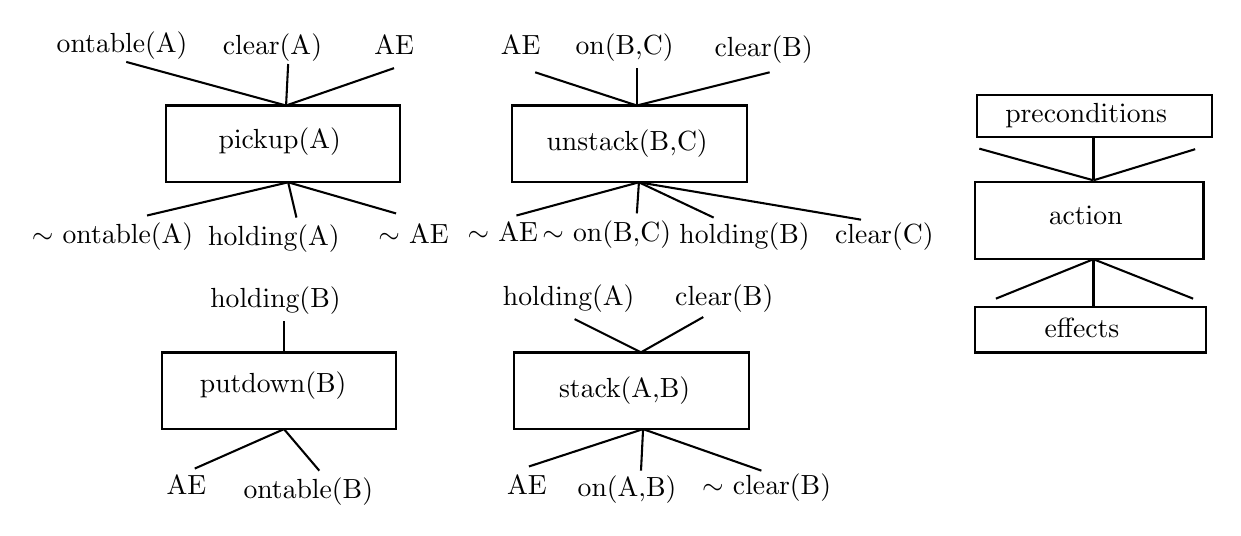
\begin{tikzpicture}[x=0.75pt,y=0.75pt,yscale=-1,xscale=1]
        %uncomment if require: \path (0,300); %set diagram left start at 0, and has height of 300
        
        %Shape: Rectangle [id:dp5282420670346548] 
        \draw   (91,82) -- (204,82) -- (204,119) -- (91,119) -- cycle ;
        %Straight Lines [id:da14751894195392823] 
        \draw    (72,61) -- (149,82) ;
        %Straight Lines [id:da743073474521007] 
        \draw    (150,62) -- (149,82) ;
        %Straight Lines [id:da5058996990400927] 
        \draw    (201,64) -- (149,82) ;
        %Straight Lines [id:da6648991704266418] 
        \draw    (82,135) -- (150,119) ;
        %Straight Lines [id:da9182943057342643] 
        \draw    (154,136) -- (150,119) ;
        %Straight Lines [id:da7510471749408582] 
        \draw    (202,134) -- (150,119) ;
        
        %Shape: Rectangle [id:dp26333691077270716] 
        \draw   (258,82) -- (371,82) -- (371,119) -- (258,119) -- cycle ;
        %Straight Lines [id:da15870535581756018] 
        \draw    (318,82) -- (269,66) ;
        %Straight Lines [id:da7550821955548243] 
        \draw    (318,64) -- (318,82) ;
        %Straight Lines [id:da5984645764220847] 
        \draw    (382,66) -- (318,82) ;
        %Straight Lines [id:da25234414353512913] 
        \draw    (260,135) -- (319,119) ;
        %Straight Lines [id:da3776381045418554] 
        \draw    (318,134) -- (319,119) ;
        %Straight Lines [id:da23306335007520695] 
        \draw    (355,136) -- (319,119) ;
        %Straight Lines [id:da8212108058076527] 
        \draw    (426,137) -- (319,119) ;
        
        %Shape: Rectangle [id:dp0423267668387286] 
        \draw   (259,201) -- (372,201) -- (372,238) -- (259,238) -- cycle ;
        %Straight Lines [id:da8870653215758376] 
        \draw    (288,184.92) -- (320,200.92) ;
        %Straight Lines [id:da45000955469333737] 
        \draw    (350,183.92) -- (320,200.92) ;
        %Straight Lines [id:da3246619478445869] 
        \draw    (266,255.92) -- (321,237.92) ;
        %Straight Lines [id:da6256221215347636] 
        \draw    (320,257.92) -- (321,237.92) ;
        %Straight Lines [id:da48935665888268887] 
        \draw    (378,257.92) -- (321,237.92) ;
        
        %Shape: Rectangle [id:dp9038522216404955] 
        \draw   (89,201) -- (202,201) -- (202,238) -- (89,238) -- cycle ;
        %Straight Lines [id:da2426183858496329] 
        \draw    (148,185.88) -- (148,200.88) ;
        %Straight Lines [id:da8710597762004703] 
        \draw    (105,256.92) -- (148,237.92) ;
        %Straight Lines [id:da09734642252119541] 
        \draw    (165,257.92) -- (148,237.92) ;
        
        %Shape: Rectangle [id:dp4549981653617977] 
        \draw   (481,119) -- (591,119) -- (591,156) -- (481,156) -- cycle ;
        
        %Shape: Rectangle [id:dp05373055193520637] 
        \draw   (481,179) -- (592,179) -- (592,201) -- (481,201) -- cycle ;
        
        %Shape: Rectangle [id:dp2694694944007495] 
        \draw   (482,77) -- (595,77) -- (595,97) -- (482,97) -- cycle ;
        
        %Straight Lines [id:da7196336250864821] 
        \draw    (483,102.78) -- (538,118.05) ;
        %Straight Lines [id:da5385936874728813] 
        \draw    (587,103.05) -- (538,118.05) ;
        %Straight Lines [id:da4482167007450657] 
        \draw    (538,97.05) -- (538,118.05) ;
        %Straight Lines [id:da7125431960902598] 
        \draw    (538,179.05) -- (538,156.05) ;
        %Straight Lines [id:da6280410433234542] 
        \draw    (538,156.05) -- (586,175.05) ;
        %Straight Lines [id:da36447110871236266] 
        \draw    (538,156.05) -- (491,175.05) ;
        
        
        % Text Node
        \draw (494,79.27) node [anchor=north west][inner sep=0.75pt]   [align=left] {preconditions};
        % Text Node
        \draw (515,129) node [anchor=north west][inner sep=0.75pt]   [align=left] {action};
        % Text Node
        \draw (513,182.89) node [anchor=north west][inner sep=0.75pt]   [align=left] {effects};
        % Text Node
        \draw (273,92) node [anchor=north west][inner sep=0.75pt]   [align=left] {unstack(B,C)};
        % Text Node
        \draw (287,46) node [anchor=north west][inner sep=0.75pt]   [align=left] {on(B,C)};
        % Text Node
        \draw (354,47) node [anchor=north west][inner sep=0.75pt]   [align=left] {clear(B)};
        % Text Node
        \draw (412,137) node [anchor=north west][inner sep=0.75pt]   [align=left] {clear(C)};
        % Text Node
        \draw (235,137) node [anchor=north west][inner sep=0.75pt]   [align=left] {$\sim$ AE};
        % Text Node
        \draw (251,47) node [anchor=north west][inner sep=0.75pt]   [align=left] {AE};
        % Text Node
        \draw (337,137) node [anchor=north west][inner sep=0.75pt]   [align=left] {holding(B)};
        % Text Node
        \draw (271,136) node [anchor=north west][inner sep=0.75pt]   [align=left] {$\sim$ on(B,C)};
        % Text Node
        \draw (115,91) node [anchor=north west][inner sep=0.75pt]   [align=left] {pickup(A)};
        % Text Node
        \draw (190,47) node [anchor=north west][inner sep=0.75pt]   [align=left] {AE};
        % Text Node
        \draw (117,46) node [anchor=north west][inner sep=0.75pt]   [align=left] {clear(A)};
        % Text Node
        \draw (37,45) node [anchor=north west][inner sep=0.75pt]   [align=left] {ontable(A)};
        % Text Node
        \draw (110,138) node [anchor=north west][inner sep=0.75pt]   [align=left] {holding(A)};
        % Text Node
        \draw (25,137) node [anchor=north west][inner sep=0.75pt]   [align=left] {$\sim$ ontable(A)};
        % Text Node
        \draw (192,138) node [anchor=north west][inner sep=0.75pt]   [align=left] {$\sim$ AE};
        % Text Node
        \draw (106,209) node [anchor=north west][inner sep=0.75pt]   [align=left] {putdown(B)};
        % Text Node
        \draw (127,260) node [anchor=north west][inner sep=0.75pt]   [align=left] {ontable(B)};
        % Text Node
        \draw (90,259) node [anchor=north west][inner sep=0.75pt]   [align=left] {AE};
        % Text Node
        \draw (111,168) node [anchor=north west][inner sep=0.75pt]   [align=left] {holding(B)};
        % Text Node
        \draw (279,211) node [anchor=north west][inner sep=0.75pt]   [align=left] {stack(A,B)};
        % Text Node
        \draw (348,258) node [anchor=north west][inner sep=0.75pt]   [align=left] {$\sim$ clear(B)};
        % Text Node
        \draw (335,167) node [anchor=north west][inner sep=0.75pt]   [align=left] {clear(B)};
        % Text Node
        \draw (254,259) node [anchor=north west][inner sep=0.75pt]   [align=left] {AE};
        % Text Node
        \draw (252,167) node [anchor=north west][inner sep=0.75pt]   [align=left] {holding(A)};
        % Text Node
        \draw (288,259) node [anchor=north west][inner sep=0.75pt]   [align=left] {on(A,B)};
        
        
        \end{tikzpicture}
        \caption{Block Worlds Domain}
    \end{figure}
\end{itemize}
\pagebreak

\subsection{Forward State Space Planning}
\begin{itemize}
    \item \textbf{Applicable actions}: Given a state $S$ and action $a$ is applicable in the state $S$ if its preconditions are satisfied in the state. That is,
    \begin{equation*}
        pre(a)\subseteq S
    \end{equation*}
    \item \textbf{Progression}: If an applicable action $a$ is applied in a state $S$ then the state transitions or progresses to a new state $S'$, defined as,
    \begin{equation*}
        S'=\gamma(S,a)=\{S\cup effects^+(a)\}\text{\textbackslash}effects^-(a)
    \end{equation*}
    \item \textbf{Plan}: A plan $\pi$ is a sequence of actions $\langle a_1,a_2,...,a_n\rangle$. A plan $\pi$ is applicable in a state $S_0$ if there are states $S_1,...,S_n$ such that $\gamma(S_{i-1},a_i)=S_i$ for $i=1,...,n$.\\
    The final state is $S_n=\gamma(S_0,\pi)$
    \item \textbf{Valid Plan}: Let $G$ be a goal description. Then a plan is a valid plan in a state $S_0$ if
    \begin{equation*}
        G\subseteq \gamma(S_0,\pi)
    \end{equation*}
    \item FSSP has a high branching factor. This is because the given state is completely described, and many actions are applicable.
\end{itemize}

\subsection{Backward State Space Planning}
\begin{itemize}
    \item \textbf{Relevant actions}: Given a goal $G$ an action $a$ is relevant to the goal if it produces some positive effect in the goal, and deletes none. That is,
    \begin{equation*}
        \{effect^+(a)\cap G\}\neq \phi \land \{effects^-(a)\cap G\}=\phi
    \end{equation*}
    \item \textbf{Regression}: If a relevant action $a$ is applied in a goal $G$ then the goal regresses to a new goal $G'$, also called a subgoal, define as
    \begin{equation*}
        G'=\gamma^{-1}(G,a)=\{G\text{\textbackslash}effects^+(a)\} \cup pre(a)
    \end{equation*}
    \item \textbf{Plan}: A plan $\pi$ is a sequence of actions $\langle a_1,a_2,...,a_n\rangle$. A plan $\pi$ is relevant to a goal $G_n$ if there are goals $G_0,...,G_{n-1}$ such that $G_{i-1}=\gamma^{-1}(G_i,a_i)$ for $i=1,...,n$\\
    The final goal is $G_0=\gamma^{-1}(G_n,\pi)$
    \item \textbf{Valid Plan}: Let $S_0$ be the start state. Regression ends when $G_0\subseteq S_0$. The plan $\pi$ is a valid plan if $G_n\subseteq \gamma(S_0,\pi)$. Validity is still checked by progression.
    \item BSSP has a lower branching factor. This is because the goal description is often quite small.
\end{itemize}

\begin{table}[H]
    \centering
    \begin{tabular}{|p{15mm}|p{60mm}|p{75mm}|}
        \hline
         & FSSP & BSSP \\
         \hline
        Start at & Start State & Goal Description\\
        \hline
        Moves & $a$ is applicable \newline $pre(a)\subseteq S$ & $a$ is relevant \newline $\{effect^+(a)\cap G\}\neq \phi \land \{effects^-(a)\cap G\}=\phi$\\
        \hline
        Transition & Progression\newline $S'=\{S\cup effects^+(a)\}\text{\textbackslash}effects^-(a)$ \newline Sound \newline $\pi \gets \pi \circ a$ & Regression \newline $G'=\{G\text{\textbackslash}effects^+(a)\} \cup pre(a)$ \newline Not Sound \newline $\pi \gets a\circ \pi$\\
        \hline
        Goal Test & $G\subseteq \gamma(S_0,\pi)$ & $\gamma^{-1}(G_n,\pi)\subseteq S_0$ \newline followed by validity check\\
        \hline
    \end{tabular}
    \caption{FSSP vs BSSP}
\end{table}
\pagebreak

\subsection{Goal Stack Planning}
\begin{itemize}
    \item Strives to combine features of FSSP and BSSP
    \item The basic idea is to break up a compound goal into individual goals and solve them serially one by one, producing a plan that is a sequence of actions, a linear plan.
    \item It is best suited to domains where goals can be solved serially one at a time.
    \item Employs a stack in which goals are pushed in a backward manner with actions that could achieve them.
    \item A basic operation in GSP is $PushSet(G)$
    \begin{enumerate}
        \item First push a compound goal $G=\{g_1,g_2,...,g_n\}$ or $\{g_1\land g_2\land ...\land g_n\}$
        \item and then the individual goals $g_1,...,g_n$ in some order
        \item to be solved in last in first out order
        \item possibility of using a heuristic function for ordering the goals or some form of reasoning.
    \end{enumerate}
    \item The reason to insert the compound goal too is to check whether after having solved the individual goals independently the compound goal has indeed been solved.
    \item The algorithm maintains the current state $S$ at all times.
    \item When a goal $g$ is popped from the stack, there are two possibilities.
    \begin{enumerate}
        \item $g\in S$, when the goal is true in the current state nothing needs to be done.
        \item $g\notin S$ when the goal is not true, push relevant action $a$ onto the stack followed by $PushSet(pre(a))$ and the individual goals in $pre(a)$ in some order.
    \end{enumerate}
    \item If an action $a$ is popped then it must be applicable and can be added to the plan.
    \begin{algorithm}[H]
        \caption{Goal Stack Planning}\label{alg:AI-GSP}
        \begin{algorithmic}[1]
            \Statex \Call{GSP}{$givenState,givenGoal,actions$}
            \State $S\gets givenState$; $plan\gets ()$; $stack\gets emptyStack$
            \State \Call{PushSet}{$givenGoal,stack$}
            \While{not \Call{Empty}{$stack$}}
                \State $x\gets \Call{Pop}{stack}$
                \If{$x$ is an action $a$}
                    \State $plan\gets (plan\circ a)$
                    \State $S\gets \Call{Progress}{S,a}$
                \ElsIf{$x$ is a compound goal $G$ and $G$ is not true}
                    \State \Call{PushSet}{$G,stack$}
                \ElsIf{$x$ is a goal $g$ and $g\notin S$}
                    \State CHOOSE a relevant action $a$ that achieves $g$
                    \If{$a$ is none} 
                        \State \Return FAILURE 
                    \EndIf
                    \State \Call{Push}{$a,stack$}
                    \State \Call{PushSet}{$pre(a),stack$}
                \EndIf
            \EndWhile
            \State \Return $plan$
        \end{algorithmic}
    \end{algorithm}
    \item Goal ordering matters, it is possible to end up in a dead end or get a longer path.
    \item Certain problems have non-serializable subgoals, there is no optimal order for solving them.
    \item We may even have to undo previous subgoals to achieve new ones.
    \item \textbf{Sussman's Anomaly}: Neither order of goals will give an optimal plan.
    \item Sussman showed that there are many problems that have non-serializable subgoals.
\end{itemize}
\pagebreak

\subsection{Plan Space Planning}
\begin{itemize}
    \item Consider the space of all possible plans, and search in this space for a plan.
    \item \textbf{Partial plans}: Search space consists of partial plans.
    \item A partial plan is a 4 tuple, $\pi=\langle A,O,L,B\rangle$
    \begin{enumerate}
        \item $A$ is a set of partially instantiated operators or actions in the plan\\
        The set simply identifies the actions that are somewhere in the plan. The actions may be partially instantiated, for example, $Stack(A,?X)$ - stack block $A$ onto some block.
        \item $O$ is a set of ordering links or relations of the form $(A_i\prec A_j)$\\
        The partial plan is thus a directed graph, it imposes an order on some actions in the plan.
        \item $L$ is a set of causal links of the form $(A_i,P,A_j)$\\
        The causal link represents fact that action $A_i$ has a positive effect $P$ which is a precondition for $A_j$. $A_i$ is the producer of $P$, and $A_j$ is the consumer of $P$.
        \item $B$ is a set of binding constraints of the form
        \begin{equation*}
            (?X=?Y),(?X\neq?Y),(?X=A),(?X\neq B),(?X\neq D_X)
        \end{equation*}
    \end{enumerate}
    \item Given a planning problem $\langle S=\{s_1,s_2,...,s_n\},G=\{g_1,g_2,...,g_k\},O\rangle$
    \item Planning in plan space always begins with an initial plan $\pi_0=\langle \{A_0,A_\infty\},\{(A_0\prec A_\infty)\},\{\},\{\}\rangle$
    \item $A_0$ is the initial action with no preconditions and whose positive effects are $s_1,s_2,...,s_n$
    \item $A_\infty$ is the final action with preconditions $g_1,g_2,...,g_k$ and no effects.
    \item A partial plan may have two kinds of flaws
    \begin{enumerate}
        \item \textbf{Open goals}: any precondition of any action in the partial plan that is not supported by a causal link
        \item \textbf{Threats}: A causal link $(A_i,P,A_j)$ is said to have a threat if there exists another action $A_t$ in the plan that potentially deletes $P$ before it can be consumed.
    \end{enumerate}
    \item Plan space planning involves systematically removing flaws.
    \item A solution plan is a partial plan without any flaws.
    \item A causal link for $P$ can be found in two ways
    \begin{enumerate}
        \item If an existing action $A_e$ produces $P$ and it is consistent to add $(A_e\prec A_p)$, then add a causal link $(A_e,P,A_p)$ and add the ordering link $(A_e\prec A_p)$ to the partial plan.
        \item If no such action can be found then insert a new action $A_{new}$ that produces $P$ to the partial plan. Add the corresponding causal link $(A_{new},P,A_p)$ and the ordering link $(A_{new}\prec A_p)$.
    \end{enumerate}
    \item \textbf{Threats Materializing}: Disruption will happen if all three of the following happen
    \begin{enumerate}
        \item $A_{threat}$ has an effect $\sim Q$ such that $P$ can be unified with $Q$.
        \item $A_{threat}$ happens after $A_i$
        \item $A_{threat}$ happens before $A_j$
    \end{enumerate}
    \item We can resolve a threat by removing one of the conditions
    \begin{enumerate}
        \item \textbf{Separation}: Ensure that $P$ and $Q$ cannot unify. This can be done by adding an appropriate binding constraint to the set $B$ in the partial plan.
        \item \textbf{Promotion}: Advance the action $A_{threat}$ to happen before it can disrupt the causal link. Add an ordering $(A_{threat}\prec A_i)$ to the set $O$ in the partial plan.
        \item \textbf{Demotion}: Delay the action $A_{threat}$ to happen after both the causal link actions. Add an ordering link $(A_j\prec A_{threat})$ to the set $O$.
    \end{enumerate}
\end{itemize}

\subsection{Multi Armed Robots}
\begin{itemize}
    \item Now we want to modify the STRIPS operators to work with two arms, Arm1 and Arm2.
    \item Now, instead of $holding(X)$ and, $AE$ we would add $holding1(X)$, $holding2(X)$ and $A1E,AE2$.
    \item Similarly, we will have different actions for each arm.
    \item Clearly adding multiple actions would be infeasible, instead we have $pickup(N,A)$, and $holding(N,X)$, where $N$ is the arm number.
    \item In $unstack(A,B)$ we did not delete $clear(A)$, this is not a problem in a single arm case, but in multi-arm case we will delete it and add it back in $stack(A,B)$.
\end{itemize}

\subsection{Means Ends Analysis}
\begin{itemize}
    \item In their seminal work on \textit{Human Problem Solving}, Newell and Simon proposed a general purpose strategy for problem solving, which they call the \textbf{General Purpose Solver (GPS)}. GPS encapsulated the heuristic approach, which they called \textbf{Means Ends Analysis}.
    \item Compare the current state with the desired state, and list the differences between them.
    \item Evaluate the differences in terms of magnitude in some way.
    \item Consult an operator-difference table
    \item Reduce the largest or most important differences first.
    \item The differences characterize the ends that need to be achieved, the operators define the means of achieving those ends.
\end{itemize}

\subsection{Algorithm Graphplan}
\begin{itemize}
    \item It first constructs a structure called a \textit{planning graph} that potentially captures all possible solutions.
    \item Then proceeds to search for a solution in the planning graph.
    \item Starting with Graphplan, a variety of new planning algorithms burst forth
    \item These algorithms increased the length of plans that could be constructed by an order of magnitude, from tens of actions to hundreds of actions.
    \item We can also try to convert the planning problem to a satisfiability or constraint satisfaction problem, then use a SAT solver or CSP solver respectively.
    \item Another direction of research was Heuristic Search planners, domain independent heuristics to guide state space search.
    \item State space search generates a successor candidate state, which will be a starting point for further exploration.
    \item The planning graph is a structure which merges the states produced by the different applicable actions.
    \item The resulting set of propositions forms a layer, as does the set of actions that resulted in this layer.
    \item The planning graph is a layered graph made up of alternating sets of action layers and proposition layer.
    \item \textbf{Action layer}: Set if all individually applicable actions.
    \item \textbf{Proposition layer} is a union of all states possible.
    \item We also have a special action no-op, which is always applicable and does nothing. It has one precondition and one positive effect. Thus, every proposition is replicated in every proposition layer.
    \item We will assume the no-op actions to be implicit in figures.
    \item Actions will be connected with previous layer with pre-condition links, and will connect to next layer with $effect^+$ and $effect^-$ links.
    \item The negative effects of actions still persist in the propositional layer because of no-op operators.
    \item Because of no-op, the actions applicable in previous layer will now be applicable in current layer as well, of course there will be additional actions as well.
    \item As a result, the action and the proposition layers grow monotonically.
    \item \textbf{Mutual Exclusion (mutex) links}: Two actions $a\in A_i$ and $b\in A_i$ are mutex is one of the following holds
    \begin{enumerate}
        \item \textbf{Competing needs}: There exists $p_a\in pre(a)$ and $p_b\in pre(b)$ such that $p_a$ and $p_b$ are mutex in the preceding layer.
        \item \textbf{Inconsistent effects}: There exists a proposition $p$ such that $p\in effects^+(a)$ and $p\in effects^-(b)$ or vice versa. The semantics of these actions in parallel are not defined. And if they are linearized, then the outcome will depend upon the order.
        \item \textbf{Interference}: There exists a proposition $p$ such that $p\in pre(a)$ and $p\in effects^-(b)$ or vice versa. Then only one linear ordering of the two actions would be feasible.
        \item There exists a proposition $p$ such that $p\in pre(a)$ and $p\in effects^-(a)$ and also $p\in pre(b)$ and $p\in effects^-(b)$. That is, the proposition is consumed by each action, and hence only one of them can be executed.
    \end{enumerate}
    \item Two propositions $p\in P_i$ and $q\in P_i$ are mutex if all combinations of actions $a,b\in A_i$ with $p\in effects^+(a)$ and $q\in effects^+(b)$ are mutex.
    \item The planning graph is made up of the following sets associated with each index $i$
    \begin{enumerate}
        \item The set of actions $A_i$ in the $i^{th}$ layer.
        \item The set of propositions $P_i$ in the $i^{th}$ layer.
        \item The set of positive effect links $PostP_i$ of actions in the $i^{th}$ layer.
        \item The set of negative effect links $PostN_i$ of actions in the $i^{th}$ layer.
        \item The set of preconditions links $PreP_i$ of actions in the $i^{th}$ layer from $P_{i-1}$.
        \item The set of action mutexes in the $i^{th}$ layer.
        \item The set of proposition mutexes in the $i^{th}$ layer.
    \end{enumerate}
    \item If two propositions are non-mutex in a layer, they will be non-mutex in all subsequent layers because of the no-op actions. Likewise for two actions that are non-mutex.
    \item In $P_0$ all propositions are non-mutex, since $P_0$ depicts the start state.
    \item The process of extending the graph continues till any one of the following two conditions is achieved.
    \begin{enumerate}
        \item The newest proposition layer contains all the goal propositions, and there is no mutex relation between any of the goal propositions.
        \item The planning graph has leveled off. This means that for two consecutive levels,
        \begin{equation*}
            P_{i-1}=P\text{ and }MuP_{i-1}=MuP_i
        \end{equation*}
        If two consecutive levels have the same set of propositions with the same set of mutex relations between them, it means that no new actions can make an appearance. Hence, if the goal propositions are not present in a levelled planning graph, they can never appear, and the problem has no solution.
    \end{enumerate}
    \item When a planning graph with all goal propositions non-mutex is found, then it is possible, but not necessary, that a valid plan might exist in the graph.
    \item The algorithm regresses to a set of sub-goals that is non-mutex, continue this process in a depth first fashion.
    \item If it cannot find a sub-goal set at some level searching backwards, backtrack and try another sub-goal set.
    \item If it reaches the layer $P_0$ at some point, then it returns the subgraph that is the shortest makespan plan.
    \item else it extends the planning graph by one more level, this happens till the planning graph by one more level.
    \item Graphplan does DFS on the planning graph.
\end{itemize}

\section{Goal Based Reasoning}
\subsection{Problem Decomposition}
\begin{itemize}
    \item Problem decomposition takes a goal directed view of problem solving.
    \item The emphasis is on breaking up a problem into smaller problems, like in backward state space planning.
    \item Primitive problems are labeled SOLVED otherwise they are LIVE and have to be refined, like in the $SSS^*$ game playing algorithm.
    \item The search space generated for solving And-Or (AO) problems can be seen as a goal tree.
    \item The nodes in the search space can have a heuristic value that is an estimate of the cost of solving the node.
    \item Edge costs indicate the cost of transforming a problem.
    \item An AO graph with mixed nodes can be converted into a graph with pure AND and OR nodes at each level.
\end{itemize}

\subsection{Algorithm $AO^*$}
\begin{itemize}
    \item At any point, the algorithm $AO^*$ maintains the graph generated so far.
    \item Every choice point in the graph has a marker, marking the best choice at that point of time.
    \item The algorithm follows the marked path leading to a set of live nodes. It refines one of the LIVE nodes by expanding it, called the \textbf{forward phase}.
    \item It backs up the cost of the best hyper arc and propagates it upwards, called the \textbf{backward phase}.
    \item If the best choice leads to a SOLVED node, then the parent node is also labeled SOLVED.
    \item The algorithm terminates when the root is labelled SOLVED.
    \item The algorithm has the following cycle
    \begin{enumerate}
        \item Starting at the root, traverse the graph along marked paths till the algorithm reaches a set of unsolved nodes $U$.
        \item Pick a node $n$ from $U$ and refine it.
        \item Propagate the revised estimate of $n$ up via all ancestors.
        \item If for a node all AND successors along the marked path are marked SOLVED, then mark it SOLVED as well.
        \item If a node has OR edges emanating from it, and the cheapest successor is marked SOLVED, then mark the node SOLVED.
        \item Terminate when the root node is marked SOLVED.
    \end{enumerate}
    \item Like, $A^*$ the algorithm $AO^*$ is also admissible when the heuristic function underestimates the actual cost.
    \item Refine the best looking partial solution till the best solution is fully refined.
    \begin{algorithm}[H]
        \caption{And-Or Algorithm Forward Phase}
        \begin{algorithmic}[1]
            \Statex \Call{$AO^*$}{start, Futility}
            \State add start to G
            \State compute $h(start)$
            \State $solved(start)\gets $ FALSE
            \While{$solved(start)=FALSE$ and $h(start)\leq$ Futility}
                \LComment{Forward Phase}
                \State $U\gets$ trace marked paths in G to a set of unexpanded nodes
                \State $N\gets$ select a node from $U$
                \State $children\gets$ \Call{Successors}{$N$}
                \If{$children$ is empty}
                    \State $h(N)\gets$ Futility
                \Else 
                    \State check for looping in the members of $children$
                    \State remove any looping members from $children$
                    \For{each $S\in children$}
                        \State add $S$ to G
                        \State compute $h(S)$
                        \If{$S$ is primitive}
                            \State $solved(S)\gets$ TRUE
                        \EndIf
                    \EndFor
                \EndIf
                \algstore{bkbreak}
        \end{algorithmic}
    \end{algorithm}
    \begin{algorithm}[H]
        \caption{And-Or Algorithm Backward Phase}
        \begin{algorithmic}[1]
                \algrestore{bkbreak}
                \LComment{Propagate Back}
                \State $M\gets \{N\}$ \LComment{set of modified nodes}
                \While{$M$ is not empty}
                    \State $D\gets$ remove deepest node from $M$
                    \State compute best cost of $D$ from its children
                    \State mark best option at $D$ as MARKED
                    \If{all nodes connected through marked arcs are solved}
                        \State $solved(D)\gets $TRUE
                    \EndIf
                    \If{$D$ has changed}
                        \State add all parents of $D$ to $M$
                    \EndIf
                \EndWhile
            \EndWhile
            \If{$solved(start)=TRUE$}
                \State \Return the marked subgraph from $start$ node
            \EndIf
            \State \Return null
        \end{algorithmic}
    \end{algorithm}
\end{itemize}

\subsection{Deduction in Logic}
\begin{itemize}
    \item Given a knowledge base(KB) which is a set of sentences assumed to be true.
    \item A move is adding a new sentence in KB by inferring from current sentences.
    \item Is a given(query) sentence goal $\alpha$ necessarily true. 
    \item \textbf{The Greek Syllogism}: Given \textit{All men are mortal} and \textit{Socrates is a man} conclude \textit{Socrates is mortal}. In general, this can be written as, Given \textit{All z are y} and \textit{x is a z} then conclude \textit{x is y}.
    \item Forward chaining in First order logic, $\forall x(Man(x)\supset Mortal(x))$ and $Man(Socrates)$ then $Mortal(Socrates)$.
    \item \textbf{Backward Chaining}: aka Deductive Retrieval, the goal need not be a specific proposition, it can have variables as well. Formulas with variables can match facts.
    \item \textbf{Conjunctive Antecedents}: A goal $(R\text{ }?x)$ and a rule $(if(and(P?x)(Q?x))(R?x))$. A goal which matches the consequent of a rule reduces to the goals in the antecedents of the rule. To solve $R$, we solve both $P$ and $Q$.
    \item We solve goal trees in a depth first manner.
\end{itemize}

\section{Rule Based Expert System}
\begin{itemize}
    \item We are looking for patterns in the domain.
    \item A \textit{rule} looks at a part of a state which matches a pattern and modifies it to result in a new state.
    \item \textbf{State}: A set of sentences in some language.
    \item \textbf{Pattern}: A subset of the sentences.
    \item We are modifying the state in a piecewise fashion.
    \item A rule associates an action with a pattern in the state.
    \begin{enumerate}
        \item also called a production.
        \item unifying format for heuristic knowledge, business rules, and actions.
        \item basis for a Turing complete programming language.
    \end{enumerate}
    \item \textbf{Declarative Programming}: The user or programmer only state the rules.
    \item \textbf{Rule Based Production Systems} contain three main components
    \begin{enumerate}
        \item \textbf{Working memory (WM)}: Represents the current state, contains a set of records or statements, known as \textbf{working memory elements(WMEs)}, it is a model of the short term memory (STM) of the problem solver.
        \item \textbf{Each rule/production}: Represents a move, has a name or an identifier. Has one or more pattern on LHS and one or more action on RHS. A model of the long term memory (LTM) of the problem solver.
        \item \textbf{Inference Engine (IE)}: Matches patterns in all rules with all WMEs, picks one matching rule to fire/execute the actions in the rule. Repeat this process till some termination criterion.
    \end{enumerate}
    \item The inference works as, Match $\to$ Resolve $\to$ Execute.
    \item The Match algorithm takes the set of rules and the set of working memory elements and generates the \textbf{conflict set}.
    \item Each element in the conflict set is a rule along with identities of matching WMEs.
    \item The \textbf{conflict} to be resolved is which rule to select from the set of matching rules.
    \item Match is the most time-consuming step of this process.
    \item Resolve selects one rule along with the matching working memory elements. It encapsulates the strategy for search.
    \item Execute implements the actions on the RHS of a rule.
    \item Actions may make changes in the working memory, which is updated.
    \item OPS5 syntax for working memory
    \begin{itemize}
        \item The data structure is a structured record.
        \item Class name with a set of attributes, Attribute names are marked by $\hat{}$
        \item The data is a collection of attribute-value pairs bunched together, Order of attributes is not important. Default values of attribute is NIL.
    \end{itemize}
    \item The working memory is a collection of working memory elements, the WMEs are indexed by a time stamp that indicates the order in which they were added to the WM.
    \item OPS5 syntax for rules
    \begin{itemize}
        \item The LHS of a rule is a set of patterns, that conform to the syntax of the WMEs.
        \item The value field in patterns can have variables and Boolean tests.
        \item There may even be negative patterns.
        \item The RHS of a rule is a set of actions.
        \item Make a new WME, Remove an existing WME, Modify = Remove + Make.
        \item Other actions like Read, Write, Load, Halt$,...$
        \item All actions happen can \textbf{concurrently}.
    \end{itemize}
    \item A rule has a match in the WM if
    \begin{itemize}
        \item Each positive pattern in the rule has a matching WME. Unsigned patterns are positive by default.
        \item There is no WME in the WM that matches a negative pattern in the rule.
    \end{itemize}
    \item A pattern in a rule matches a WME in the WM if
    \begin{itemize}
        \item The class name of the pattern = class name of the WME.
        \item Each attribute condition in the pattern matches the attribute value in the WME.
        \item Attributes not mentioned in the pattern but present in the WME are ignored.
        \item $\{\}$ represent conjunction of tests, all must match.
        \item $<<>>$ represent disjunction of tests, some must match.
    \end{itemize}
    \item Given a large set of WMEs, the rule may match many pairs of elements.
    \item The set of matching rules with data is called the \textbf{conflict set(CS)}.
    \item The Inference Engine selects one rule from the conflict set.
    \item \textbf{Conflict Resolution}: Choosing which rule to execute or fire next.
    \item \textbf{Refactoriness}: A rule instance may fire only once with a set of matching WMEs. This is particularly relevant when the selected rule does not modify the WMEs matching its preconditions, else only this rule would keep firing.
    \item \textbf{Lexical Order}: All the rules that have matching instances, then choose the first one that the user has stated. And if a rule has multiple instances with different data, then choose the instance that matches the earlier data.\\
    The strategy places the onus of this choice on the user. The user is more like a programmer. This strategy is used in the programming language Prolog.\\
    Prolog thus deviates from the idea of declarative programming envisaged by pure logic programming, in which the user would only state the relation between input and output.
    \item \textbf{Specificity}: All the rules that have matching instances, then choose the instance of the rule that is most specific. Specificity can be measured in terms of the number of tests that patterns in rules need.\\
    The intuition is that the more specific the conditions of a rule are, the more appropriate the rule is likely to be in the given situation. This can facilitate default reasoning.
    \item \textbf{Recency}: All the rules that have matching instances. then choose the instance that has the most recent WME. Recency can be implemented by looking at the time stamps of the matching WMEs.\\
    The intuition is that when a problem solver adds a new element to the working memory, then any rule that matches that WME should get priority. Recency facilitates "a chain of thought" in reasoning.\\
    The conflict set can be maintained as a priority queue.
    \item \textbf{Means Ends Analysis}: The idea is to partition the set of rules based on the context and focus on one partition at a time. One can think of each partition as solving a specific subgoal or reducing a specific difference.\\
    The context is set by the first pattern in a rule. All rules in the same pattern have the same first pattern.\\
    The MEA strategy applies Recency to the first pattern in each rule, and Specificity for the remaining patterns.
    \item \textbf{Rete Net}: Looks at changes in WM and outputs changes in conflict set.
    \item \textbf{Discrimination Trees}: A popular approach to work with large amount of data is to use the Divide and Conquer approach and route the query or data token via a sequence of tests, a simple example is Binary Search Trees.
    \item Alpha nodes serve as the WM of the Rule Based System.
    \item A WME-token is inserted at the root, $<+WME>$ for an ADD action and $<-WME>$ for a DELETE action.
    \item The first test, usually, looks at the class-name and separates the tokens. Subsequent tests look at the value of some attribute.
    \item The key is to sequence the tests in such a manner so that the common tests in different patterns are higher up in the network, and shared between patterns.
    \item Test at current node, Edges mark test value.
    \item If a WME passes a test, then it moves to an appropriate alpha node at the next level, else it gets stuck on the parent node.
    \item Beta nodes have at least one parent, but generally have tow or more parents. All parents must satisfy a join condition, the shared variable must have the same value.
    \item A rule instance can be attached to any beta node.
    \item When a positive token is dropped in, it travels down, and may trigger some rules whose other conditions have already been met. If it does, then put these rule instances in a bucket, equal recency.
    \item For every rule instance in the conflict set, the sum of the lengths of the paths defines specificity. For specificity, we maintain a priority queue on the sum of lengths.
    \item Once a rule instance is selected to fire, it is removed from the conflict set, refactoriness is automatic.
    \item When a negative token is dropped in, it may go and exorcise some rules matching earlier.
    \item Rules with negative patterns need special treatment.
\end{itemize}

\section{Constraint Satisfaction Problems}
\subsection{Introduction}
\begin{itemize}
    \item A Constraint Satisfaction Problem is a triple <$X,D,C$>, also called a constraint network.
    \item $X$ is a set of variable names.
    \item $D$ is a set of domains, one for each variable.
    \item $C$ is a set of relations on subsets of variables.
    \item A solution is an assignment of values for all the variables such that all the constraints are satisfied.
    \item A network $\mathcal{R}$ is said to express a solution relation $\rho$.
    \item Every CSP can be represented as a constraint graph.
    \item A search algorithm may order variables based on the size of their domain, a heuristic.
    \item and also do propagation, reasoning, alongside.
    \item \textbf{Interpreting Line Drawings}: Four types of edges
    \begin{itemize}
        \item Arrow indicates material is on the right, $\to$ or $\gets$.
        \item Convex edge $+$, materials are at an angle of $\leq 90\deg$, pops out.
        \item Concave edge $-$, materials are at an angle of $\geq 180\deg$, like hollow.
    \end{itemize}
    \item $18$ types of joints possible
    \begin{figure}[H]
        \centering
        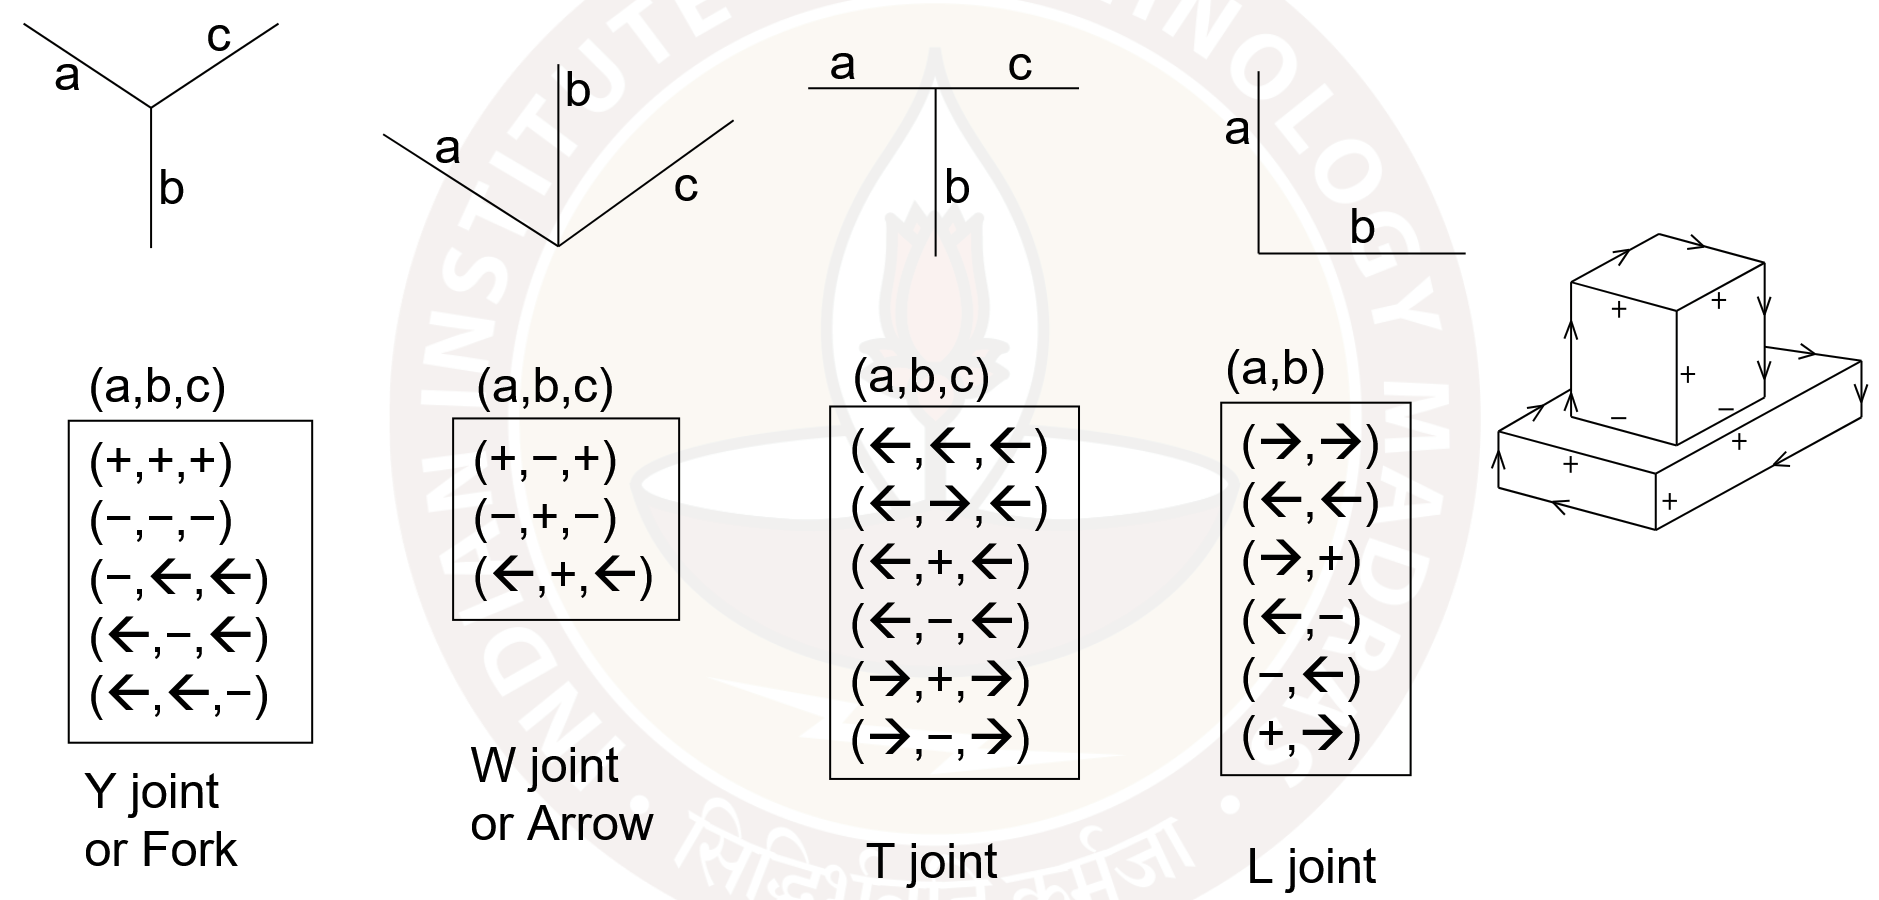
\includegraphics[width=0.8\linewidth]{Degree/static/AI_interpreting_line_drawing.png}
        \caption{Types of Joints}
    \end{figure}
    \item Two vertices have the same edge, so one label must be the same.
\end{itemize}

\subsection{Posing and Solving CSPs}
\begin{itemize}
    \item An assignment $A_Z$ assigns values to a subset $Z$ of variables, $Z\subseteq X$
    \item Let $\mathcal{A}=<a_Z,a_{Z-1},...,a_1>$ be the tuple of values in $A$.
    \item Let $\mathcal{A}_S$ be the projection of $\mathcal{A}$ on the set of variables $S$.
    \item Then $A_Z$ satisfies a constraint $C=(S,R)$ where $S$ is the scope of $R$, i.e., if $S\subseteq Z$ and $\mathcal{A}_S\in R$
    \item An assignment $A_Z$ is consistent, if for every constraint $C=(S,R)$, $A_Z$ satisfies $C$.
    \item A solution is a consistent assign for all the variables in $X$.
    \item Let $X=(x_1,x_2,...,x_N)$ be the order in which the $N$ variables are tried.
    \item Let $D_i=(a_{i1},a_{i2},...,a_{iN})$ be the values in domain $D_i$ in the order they will be tried.
    \item The search algorithm, Backtracking, is as follows
    \begin{algorithm}[H]
        \caption{Backtracking}
        \begin{algorithmic}[1]
            \Statex \Call{Backtracking}{$X,D,C$}
            \State $\mathcal{A}\gets$ [ ]
            \State $i\gets 1$
            \State $D_i'\gets D_i$
            \While{$1\leq i\leq N$}
                \State $a_i\gets \Call{SelectValue}{D_i',\mathcal{A},C}$
                \If{$a_i=$ null}
                    \State $i\gets i-1$
                    \State $\mathcal{A}\gets$ tail $\mathcal{A}$
                \Else
                    \State $\mathcal{A}\gets a_i:\mathcal{A}$
                    \State $i\gets i+1$
                    \If{$i\leq N$}
                        \State $D_i'\gets D_i$
                    \EndIf
                \EndIf
            \EndWhile
            \State \Return \Call{Reverse}{$\mathcal{A}$}
            \Statex
            \Statex \Call{SelectValue}{$D_i',\mathcal{A},C$}
            \While{$D_i'$ is not empty}
                \State $a_i\gets$ head $D_i'$
                \State $D_i'\gets$ tail $D_i'$
                \If{\Call{Consistent}{$a_i:\mathcal{A}$}}
                    \State \Return $a_i$
                \EndIf
            \EndWhile
            \State \Return null
        \end{algorithmic}
    \end{algorithm}
    \item There are various ways to combat combinatorial explosion
    \begin{enumerate}
        \item Choosing an appropriate ordering of nodes, Min-induced-width ordering of the constraint graph, Select nodes with higher degree first.
        \item Dynamic Variable Ordering, Choose variables with the smallest domains first.
        \item Preprocess the network to prune the search space, Consistency enforcement.
        \item Prune the domains during the search, Lookahead search.
        \item Intelligent Backtracking, Lookback Search, Memoization, i.e., remember combination of nodes that cannot be solved, called nogoods.
    \end{enumerate}
    \item \textbf{Arc Consistency}: Let $(X,Y)$ be an edge in the constraint graph of a network. A variable $X$ is said to be arc-consistent w.r.t variable $Y$ iff for every value $a\in D_x$ there is a value $b\in D_Y$ such that $<a,b>\in R_{XY}$\\
    $X$ can be made arc-consistent w.r.t $Y$ by algorithm Revise.
    \begin{algorithm}[H]
        \caption{Arc Consistency}
        \begin{algorithmic}[1]
            \Statex \Call{Revise}{$(X),Y$}
            \For{every $a\in D_x$}
                \If{there is no $b\in D_y$ such that $<a,b>\in R_{XY}$}
                    \State delete $a$ from $D_X$
                \EndIf
            \EndFor
        \end{algorithmic}
    \end{algorithm}
    \item An edge $(X,Y)$ is said to be arc-consistent if both $X$ and $Y$ are arc-consistent w.r.t each other.
    \item A network is arc-consistent if all its edges are arc-consistent.
    \item One cycle of calls to Revise is not enough.
    \item The algorithm $AC1$ cycles through all edges as long as even one domain changes
    \begin{algorithm}[H]
        \caption{AC1}
        \begin{algorithmic}[1]
            \Statex \Call{AC-1}{$X,D,C$}
            \Repeat
                \For{each edge $(X,Y)$ in the constraint graph}
                    \State \Call{Revise}{$(X),Y$}
                    \State \Call{Revise}{$(Y),X$}
                \EndFor
            \Until{no domain changes in the cycle}
        \end{algorithmic}
    \end{algorithm}
    \item In the worst case, the network is not arc-consistent and in every cycle exactly one element in one domain is removed.
    \item For some networks, arc-consistency results in backtrack-free search.
    \item If the domain of a variable $P$ has changed, then consistency w.r.t $P$ is enforced for the neighbors of $P$.
    \begin{algorithm}[H]
        \caption{AC3}
        \begin{algorithmic}[1]
            \Statex \Call{AC-3}{$X,D,C$}
            \State $Q\gets$ [ ]
            \For{each edge $(N,M)$ in the constraint graph}
                \State $Q\gets Q++(N,M):[(M,N)]$
            \EndFor
            \While{$Q$ is not empty}
                \State $(P,T)\gets$ head $Q$
                \State $Q\gets$ tail $Q$
                \State \Call{Revise}{$(P),T$}
                \If{$D_P$ has changed}
                    \For{each $R\neq T$ and $(R,P)$ in the constraint graph}
                        \State $Q\gets Q++[(R,P)]$
                    \EndFor
                \EndIf
            \EndWhile
        \end{algorithmic}
    \end{algorithm}
    \item A network is said to be $i$-consistency if an assignment to any $(i-1)$ variables can be consistently extended to $i$ variables.
    \item 1-consistency is also called node consistency, satisfying that a Boolean variable $P$ to a particular value.
    \item 2-consistency is called arc consistency.
    \item 3-consistency is also called path consistency, any edge in the matching diagram can be extended to a triangle.
    \item If network is strong $n$-consistent, then it also $n-1$-consistent, $n-2$-consistent,$...$.
    \item The higher the level of consistency, the lower the amount of backtracking that the search algorithm does.
    \item Achieving $i$-consistency before embarking upon search results in a smaller search space being explored.
    \item Lookahead search variations inspect all values to estimate which one would lead to fewer conflicts in the nature.
    \item Forward Checking does the least amount of work in looking ahead.
    \item Partial, Full, Arc Consistency Lookahead do increasingly more work.
    \item Arc Consistency Lookahead implements full arc consistency between the future variables.
    \item Backtracking does chronological backtracking.
    \item Jumpback methods aim to identify culprit variables, the cause of the deadend.
    \item Culprit can be identified based on graph topology or based on values that cause the conflict.
    \item Constraint programming offers a unified framework in which search and reasoning can be combined.
    \item The more the reasoning, the less the search.
    \begin{algorithm}[H]
        \caption{Forward Checking}
        \begin{algorithmic}[1]
            \Statex \Call{ForwardChecking}{$X,D,C$}
            \State $\mathcal{A}\gets$ [ ]
            \For{$k\gets 1$ to $N$}
                \State $D_k'\gets D_k$
            \EndFor
            \State $i\gets 1$
            \While{$1\leq i\leq N$}
                \State $a_i\gets \Call{SelectValue-FC}{D_i',\mathcal{A},C}$
                \If{$a_i=$ null}
                    \State Undo lookahead pruning done while choosing $a_i$
                    \State $i\gets i-1$
                    \State $\mathcal{A}\gets$ tail $\mathcal{A}$
                \Else
                    \State $\mathcal{A}\gets a_i:\mathcal{A}$
                    \State $i\gets i+1$
                \EndIf
            \EndWhile
            \State \Return \Call{Reverse}{$\mathcal{A}$}
            \Statex
            \Statex \Call{SelectValue-FC}{$D_i',\mathcal{A},C$}
            \While{$D_i'$ is not empty}
                \State $a_i\gets$ head $D_i'$
                \State $D_i'\gets$ tail $D_i'$
                \For{$k\gets i+1$ to $N$}
                    \For{each $b$ in $D_k'$}
                        \If{not \Call{Consistent}{$b:a_i:\mathcal{A}$}}
                            \State delete $b$ from $D_k'$
                        \EndIf
                    \EndFor
                \EndFor
                \If{no $D_k'$ is empty}
                    \State \Return $a_i$
                \Else
                    \For{$k\gets i+1$ to $N$}
                        \State undo deletes in $D_k'$
                    \EndFor
                \EndIf
            \EndWhile
            \State \Return null
        \end{algorithmic}
    \end{algorithm}
    
\end{itemize}


\end{document}